\chapter{Additional Measurements}
\label{app:meas}

\section{Test 1 - CCNx Throughput and Overhead}
\label{app:res-throughput-overhead}

\begin{figure}[H]

    \centering
    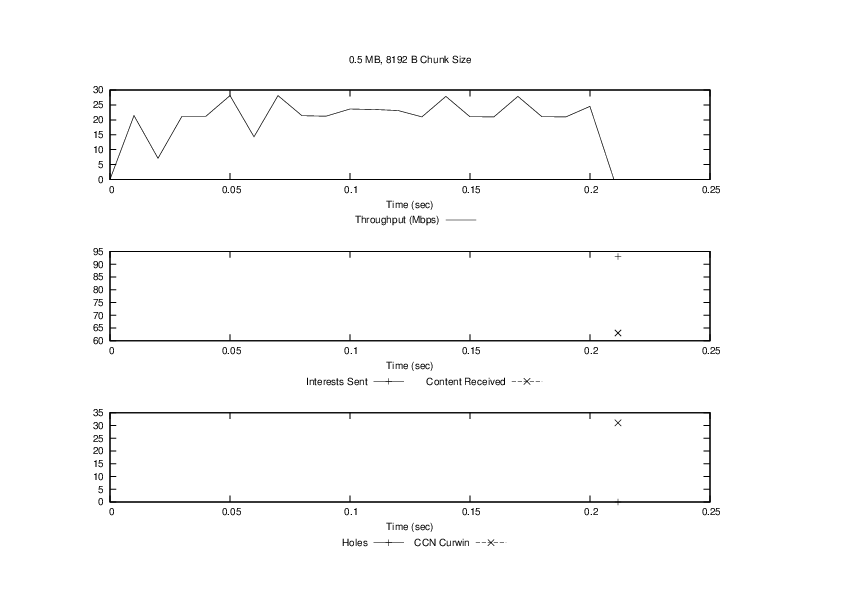
\includegraphics[width=0.75\textwidth]{figures/udp_0_5_8192.pdf}
    \cprotect\caption{Results for Test 1: Throughput in Mbps, as perceived by 
        PC1, when retrieving a file of size 500\,kB with a 8192 byte 
        `chunk' size. Statistics specific to the \verb+ccncatchunks2+ application 
        are also shown.}
    \label{fig:test-1-thpt-0_5-8192}

\end{figure}

\begin{figure}[H]

    \centering
    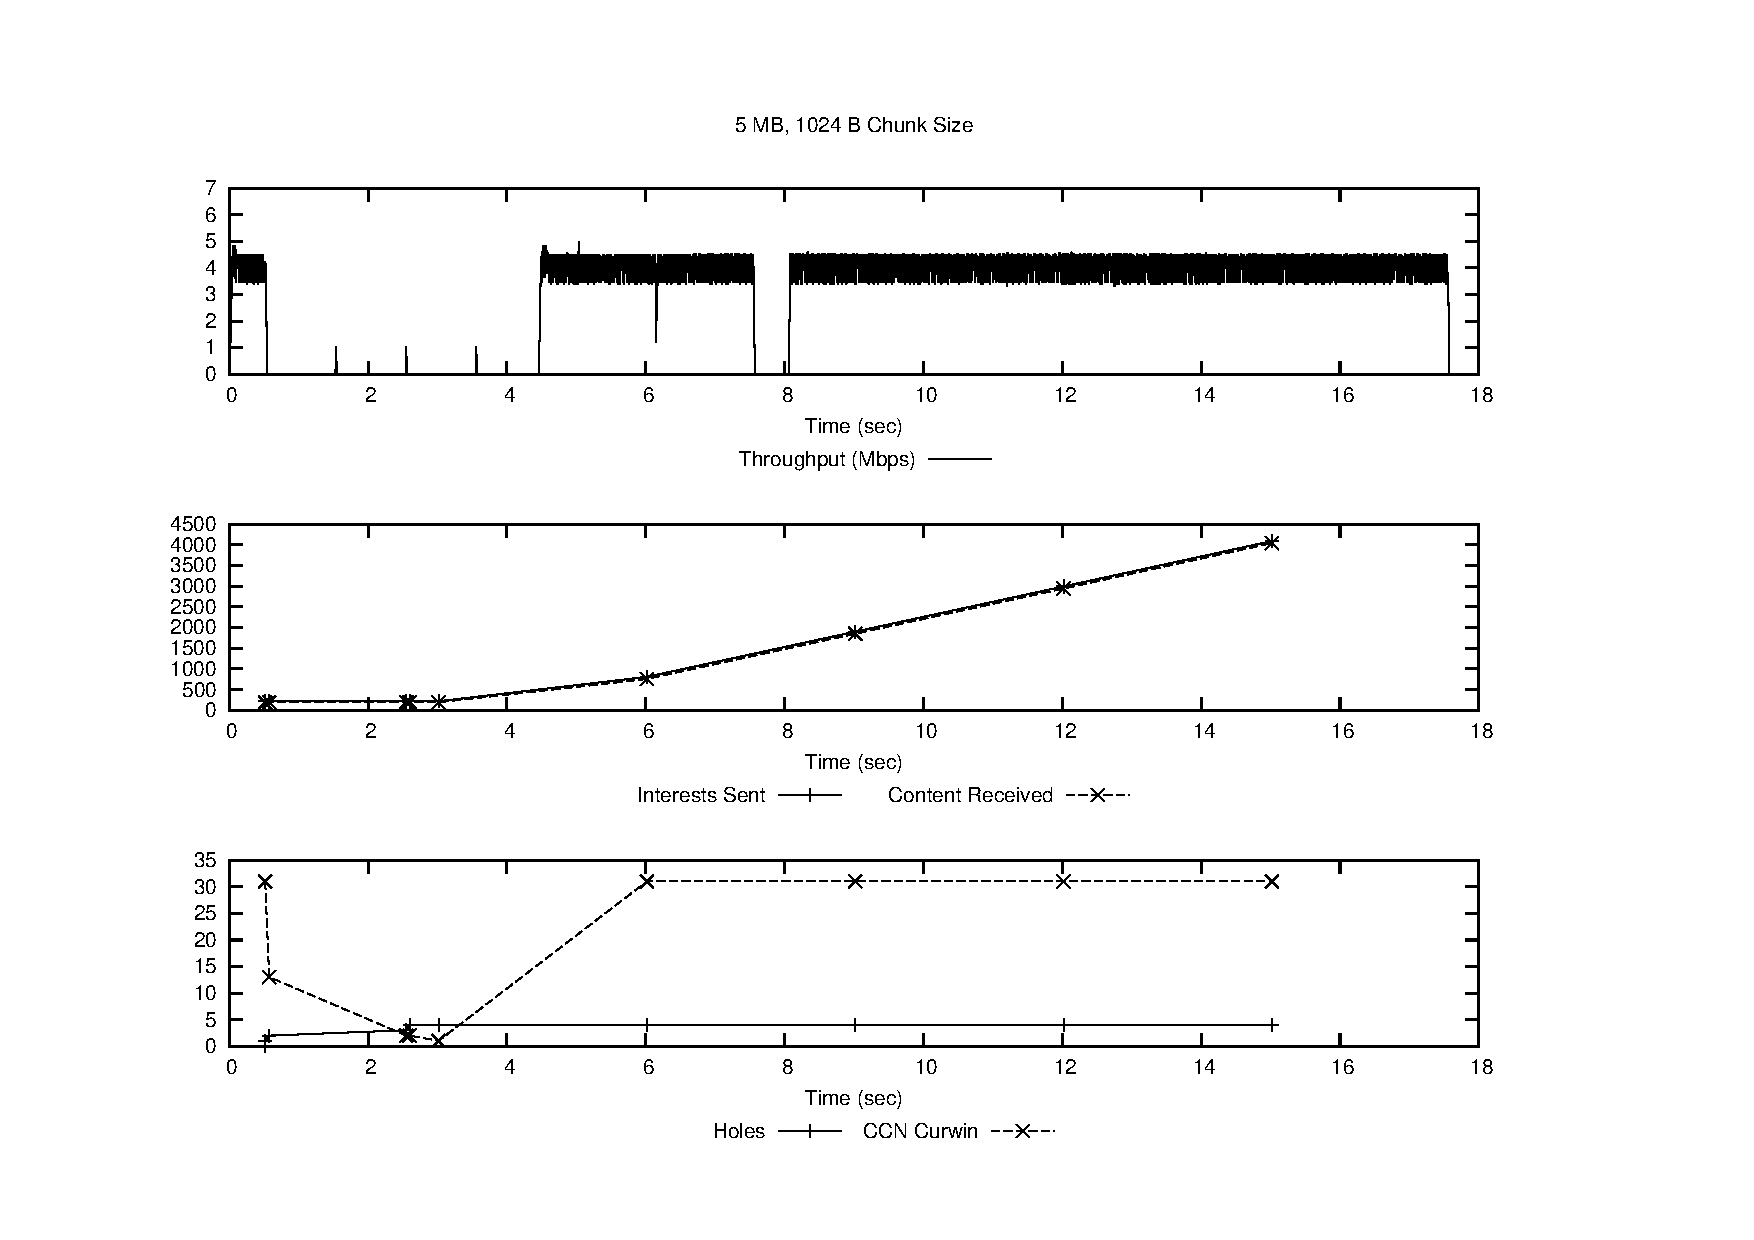
\includegraphics[width=0.75\textwidth]{figures/udp_5_1024.pdf}
    \cprotect\caption{Results for Test 1: Throughput in Mbps, as perceived by 
        PC1, when retrieving a file of size 5\,MB with a 1024 byte 
        `chunk' size. Statistics specific to the \verb+ccncatchunks2+ application 
        are also shown.}
    \label{fig:test-1-thpt-5-1024}

\end{figure}

\begin{figure}[H]

    \centering
    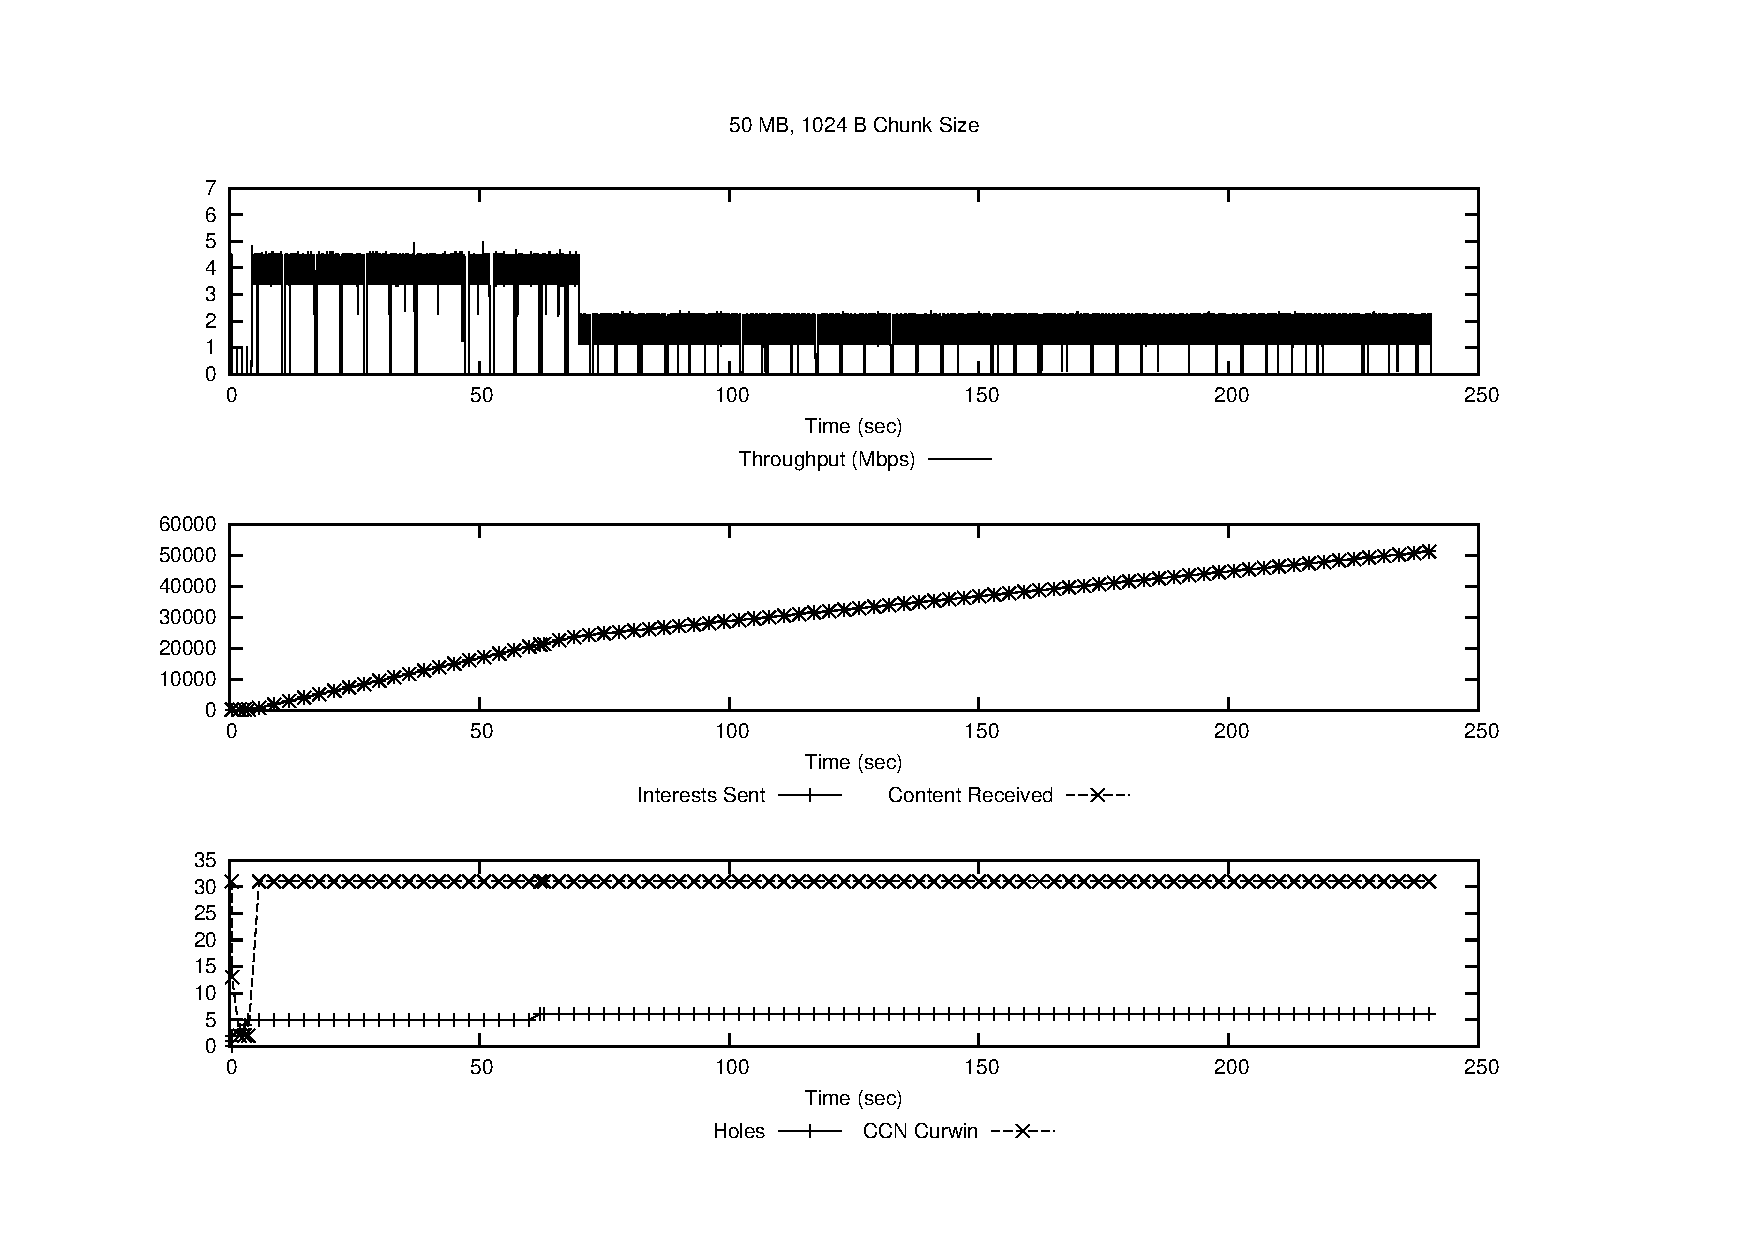
\includegraphics[width=0.75\textwidth]{figures/udp_50_1024.pdf}
    \cprotect\caption{Results for Test 1: Throughput in Mbps, as perceived by 
        PC1, when retrieving a file of size 50\,MB with a 1024 byte 
        `chunk' size. Statistics specific to the \verb+ccncatchunks2+ application 
        are also shown.}
    \label{fig:test-1-thpt-50-1024}

\end{figure}

\begin{figure}[H]

    \centering
    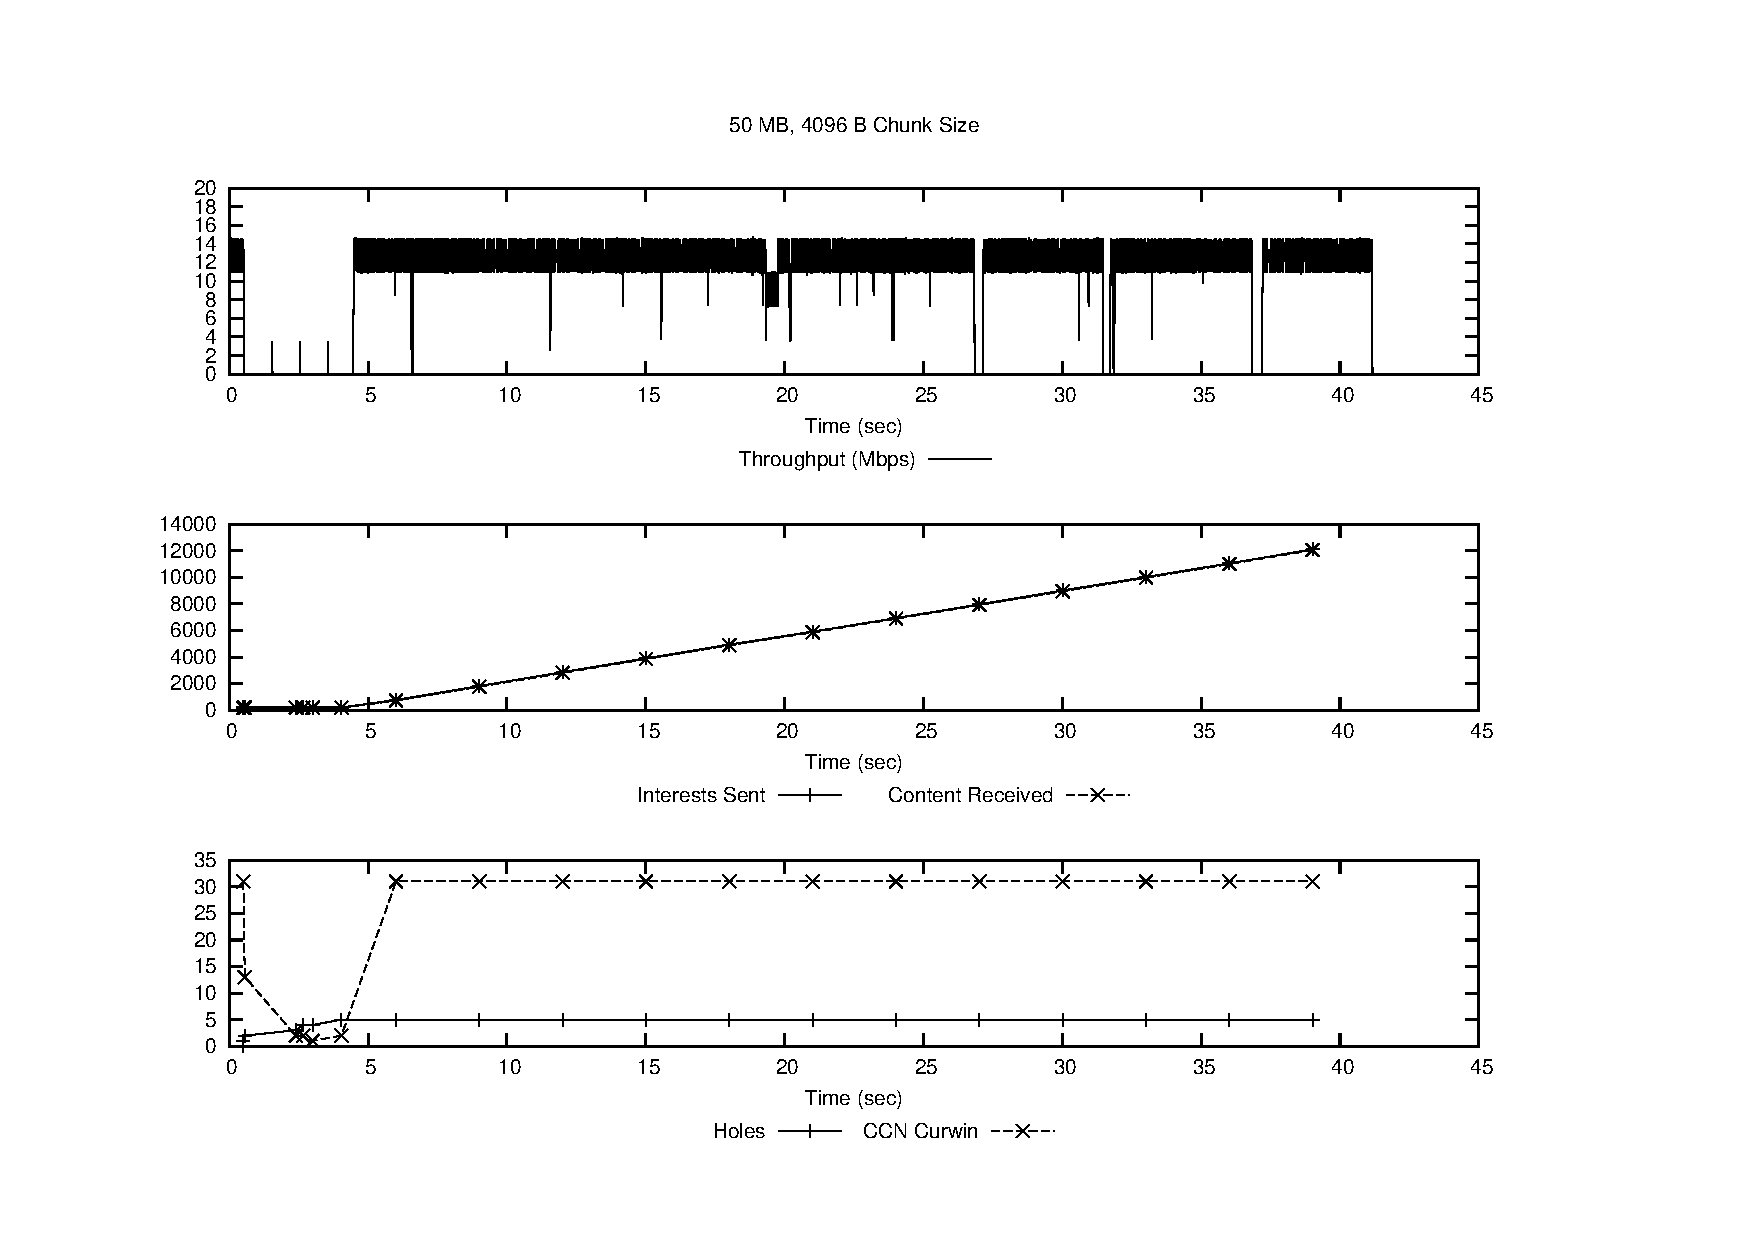
\includegraphics[width=0.75\textwidth]{figures/udp_50_4096.pdf}
    \cprotect\caption{Results for Test 1: Throughput in Mbps, as perceived by 
        PC1, when retrieving a file of size 50\,MB with a 4096 byte 
        `chunk' size. Statistics specific to the \verb+ccncatchunks2+ application 
        are also shown.}
    \label{fig:test-1-thpt-50-4096}

\end{figure}

\begin{figure}[H]

    \centering
    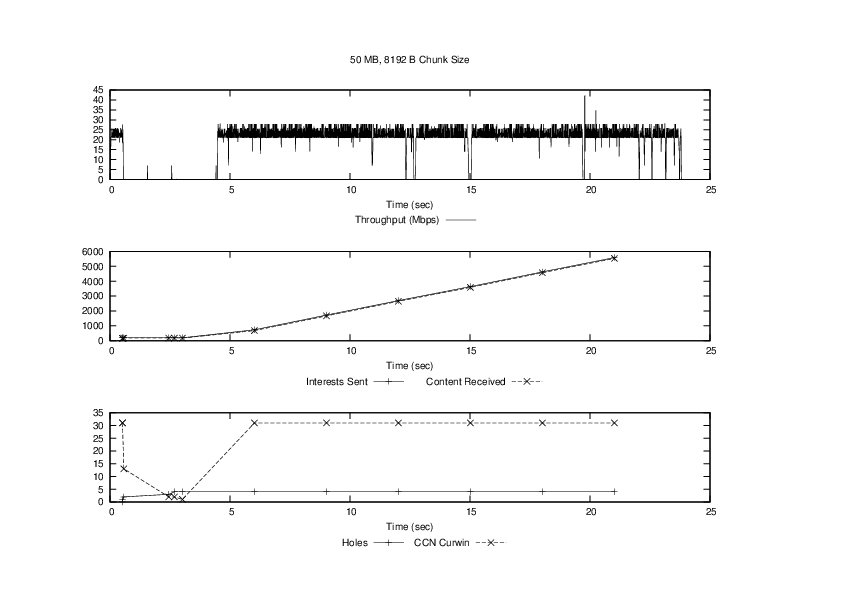
\includegraphics[width=0.75\textwidth]{figures/udp_50_8192.pdf}
    \cprotect\caption{Results for Test 1: Throughput in Mbps, as perceived by 
        PC1, when retrieving a file of size 50\,MB with a 8192 byte 
        `chunk' size. Statistics specific to the \verb+ccncatchunks2+ application 
        are also shown.}
    \label{fig:test-1-thpt-50-8192}

\end{figure}

\begin{figure}[H]

    \centering
    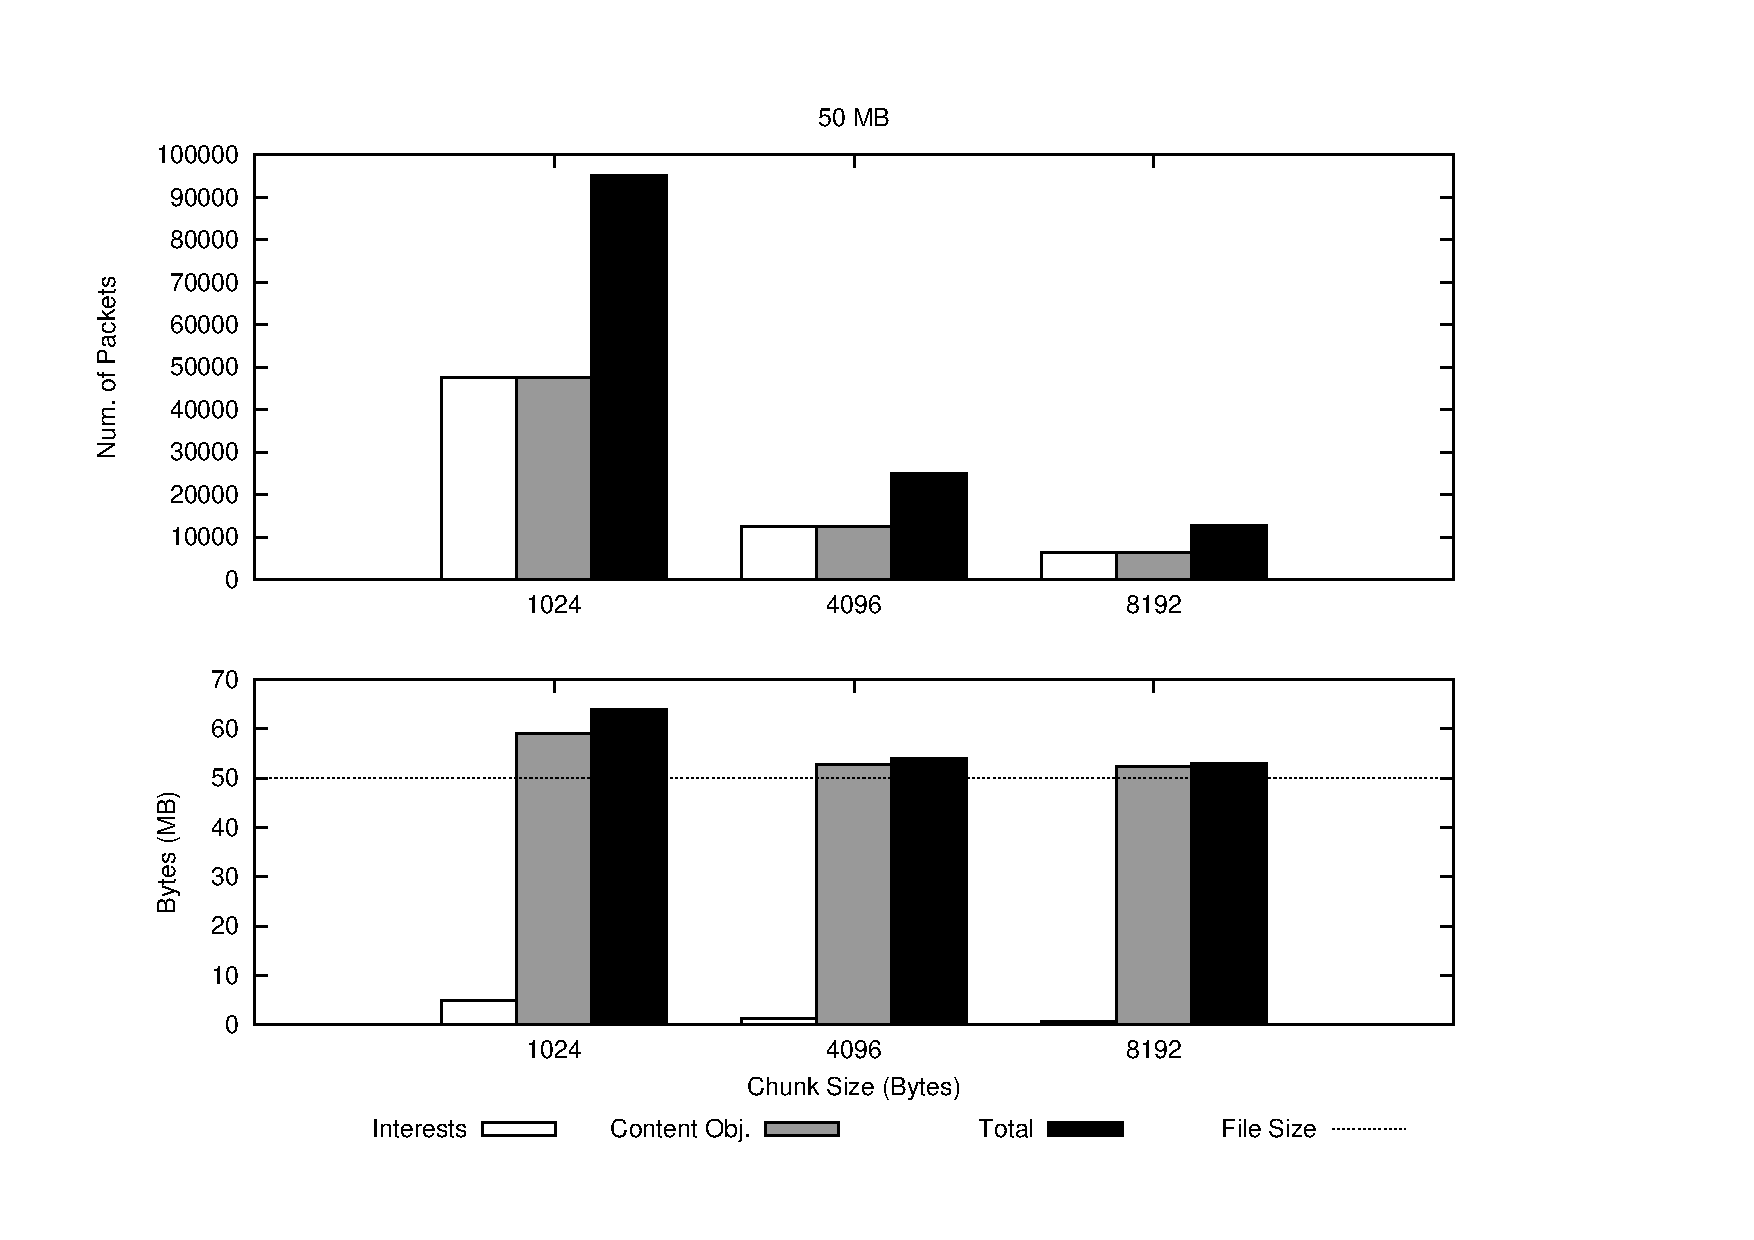
\includegraphics[width=0.75\textwidth]{figures/udp_50.pdf}
    \cprotect\caption{Results for Test 1: Packet and byte quantities, measured 
        at PC1, for a file size of 50\,MB.}
    \label{fig:test-1-packets-bytes-50}

\end{figure}

\begin{figure}[H]

    \centering
    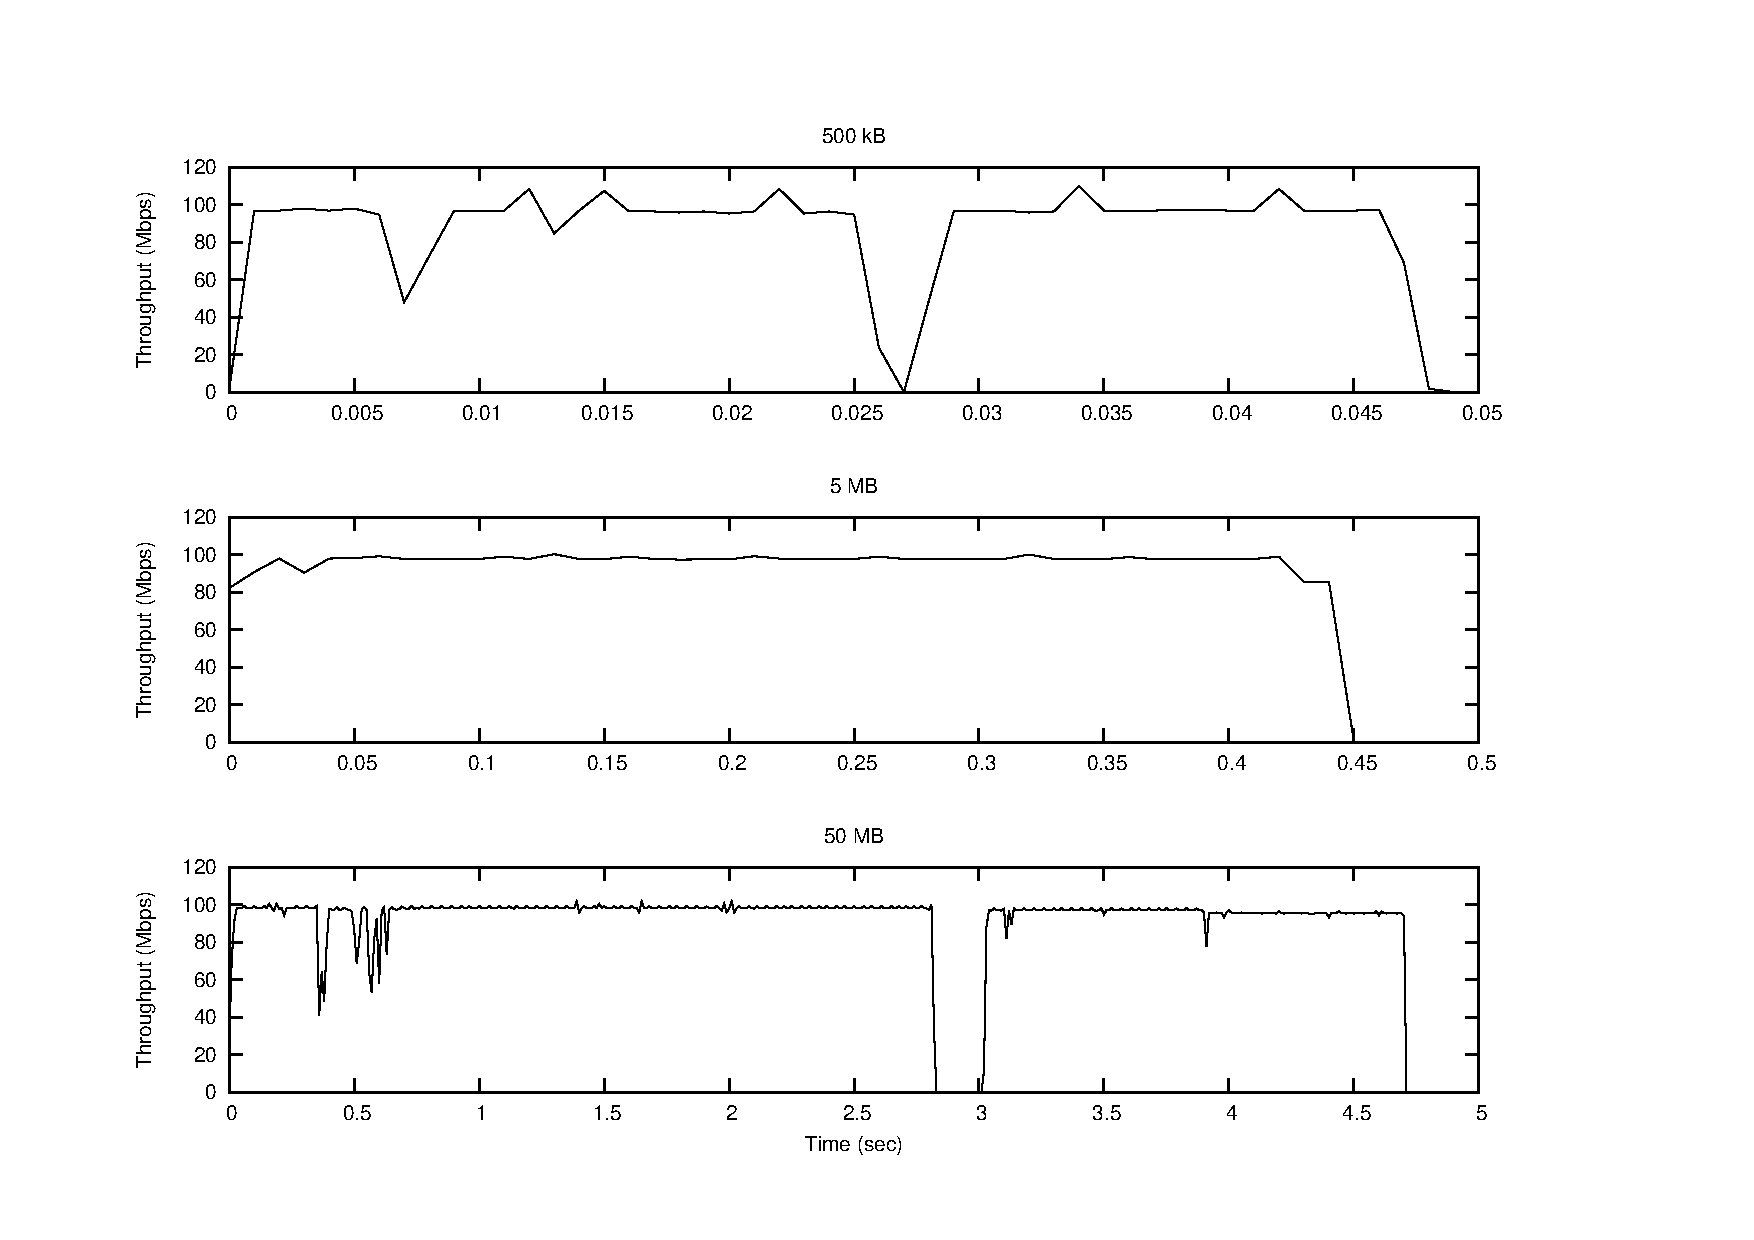
\includegraphics[width=0.75\textwidth]{figures/ftp-thpt.pdf}
    \cprotect\caption{Results for Test 1: Throughput in Mbps, as perceived by 
        PC1, when retrieving files of sizes 500\,kB, 5\,MB and 50\,MB, over 
        FTP.}
    \label{fig:test-1-thpt-ftp}

\end{figure}

\begin{figure}[H]

    \centering
    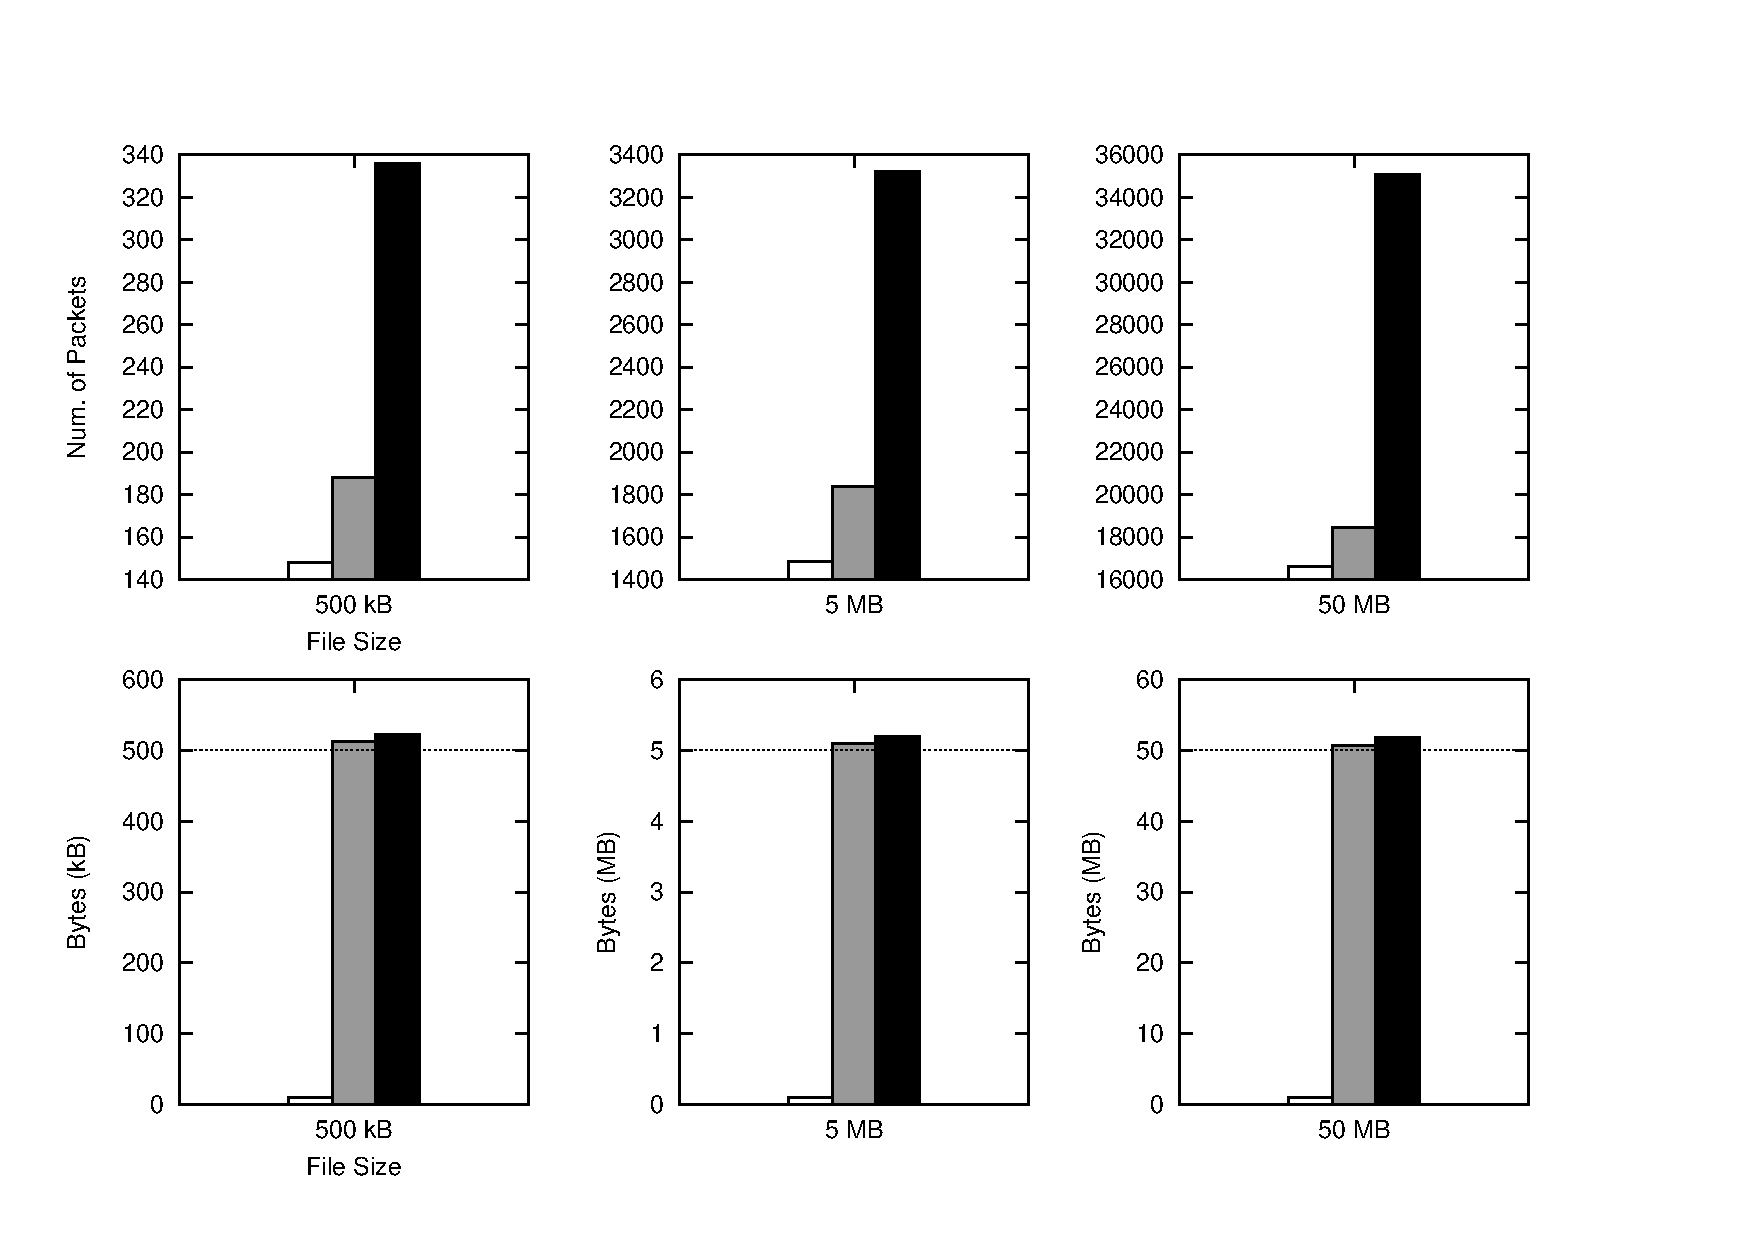
\includegraphics[width=0.75\textwidth]{figures/tcp.pdf}
    \cprotect\caption{Results for Test 1: Packet and byte quantities, measured 
        at PC1, for files of sizes 500\,kB, 5\,MB and 50\,MB, over 
        FTP. The white bars represent packets sent from the FTP client side, 
        gray represent packets sent from the FTP server side, while the 
        black bars represent the total number of exchanged packets.}
    \label{fig:test-1-packets-bytes-ftp}

\end{figure}

\section{Test 2 - CCNx Multihop Forwarding}
\label{app:res-multihop-for}

\subsection{Test 2.1 - CCNx Multihop Forwarding (File Transfer)}
\label{subapp:test-multihop-file}

\begin{figure}[H]
    \centering

    \subfigure[]{
        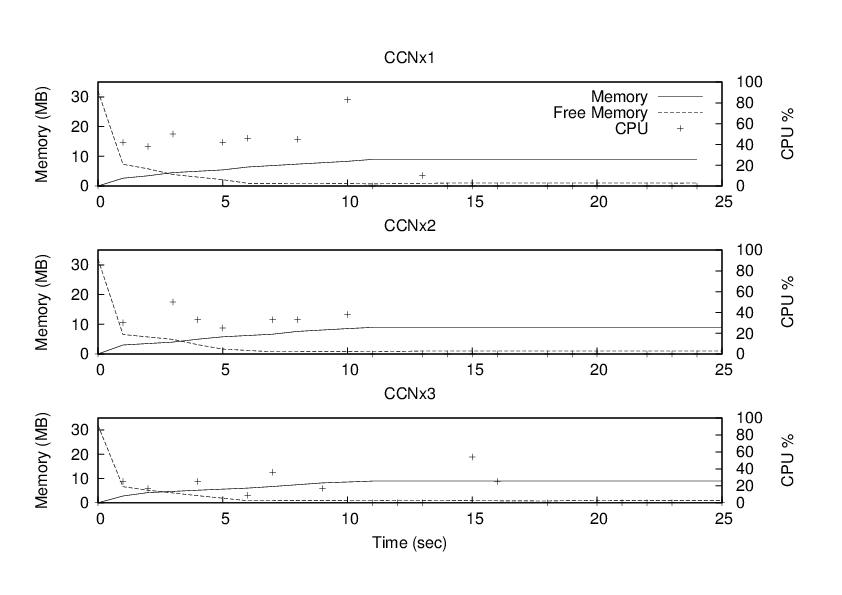
\includegraphics[width=0.75\textwidth] {figures/file_5-sep-cpu-mem.pdf}
        \label{subfig:file_5-sep-cpu-mem}
    }

    \subfigure[]{
        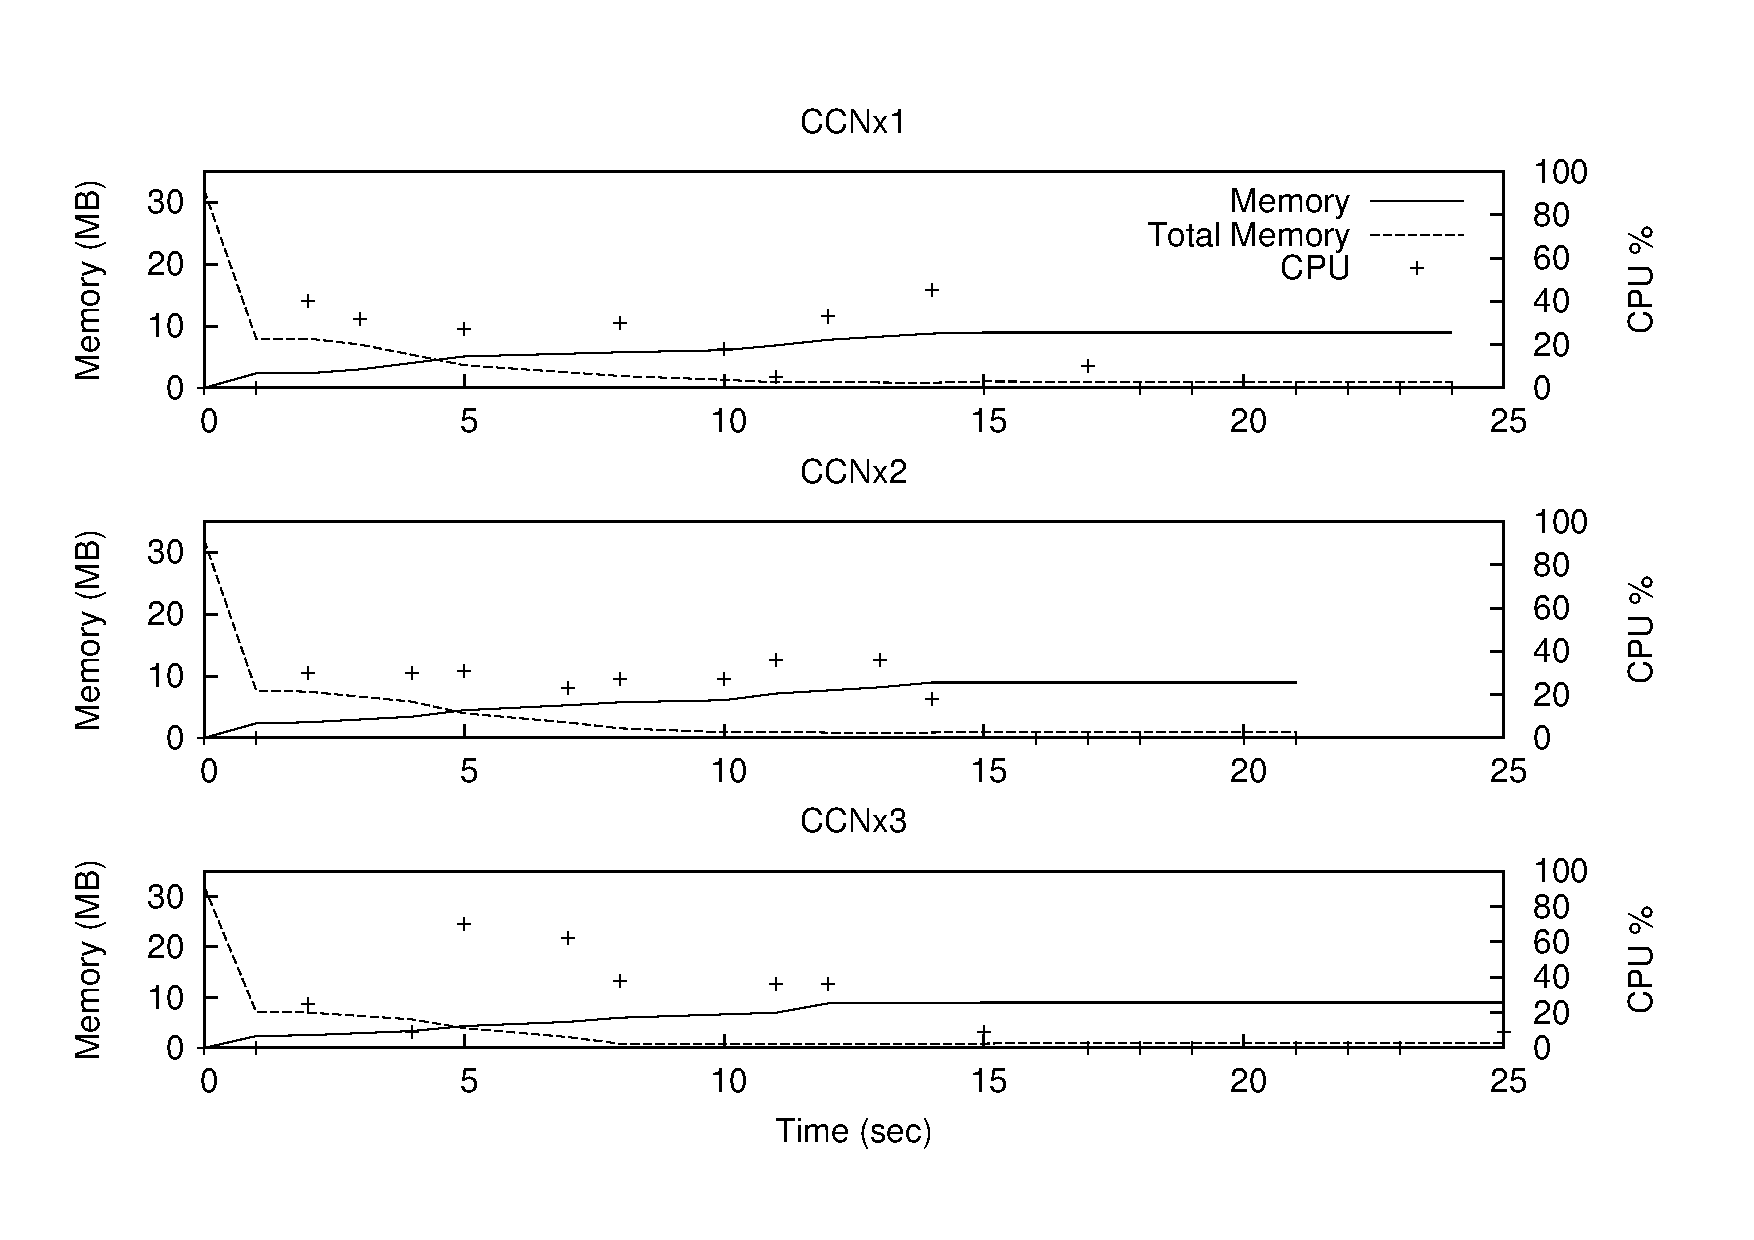
\includegraphics[width=0.75\textwidth] {figures/file_5-sim-cpu-mem.pdf}
        \label{subfig:file_5-sim-cpu-mem}
    }

    \cprotect\caption{Results for Test 2.1: CPU and memory utilization at 
        all CCNx nodes, during the transfer of a file of size 
        5\,MB, for both non-overlapping (a) and overlapping (b) cases. Regarding the 
        memory values, the `memory' line corresponds to the amount of RAM 
        occupied by the \verb+ccnd+ process, while the `free memory' corresponds 
        to the amount of free memory in the system.}
    \label{fig:file_5-cpu-mem}

\end{figure}

\begin{figure}[H]
    \centering

    \subfigure[]{
        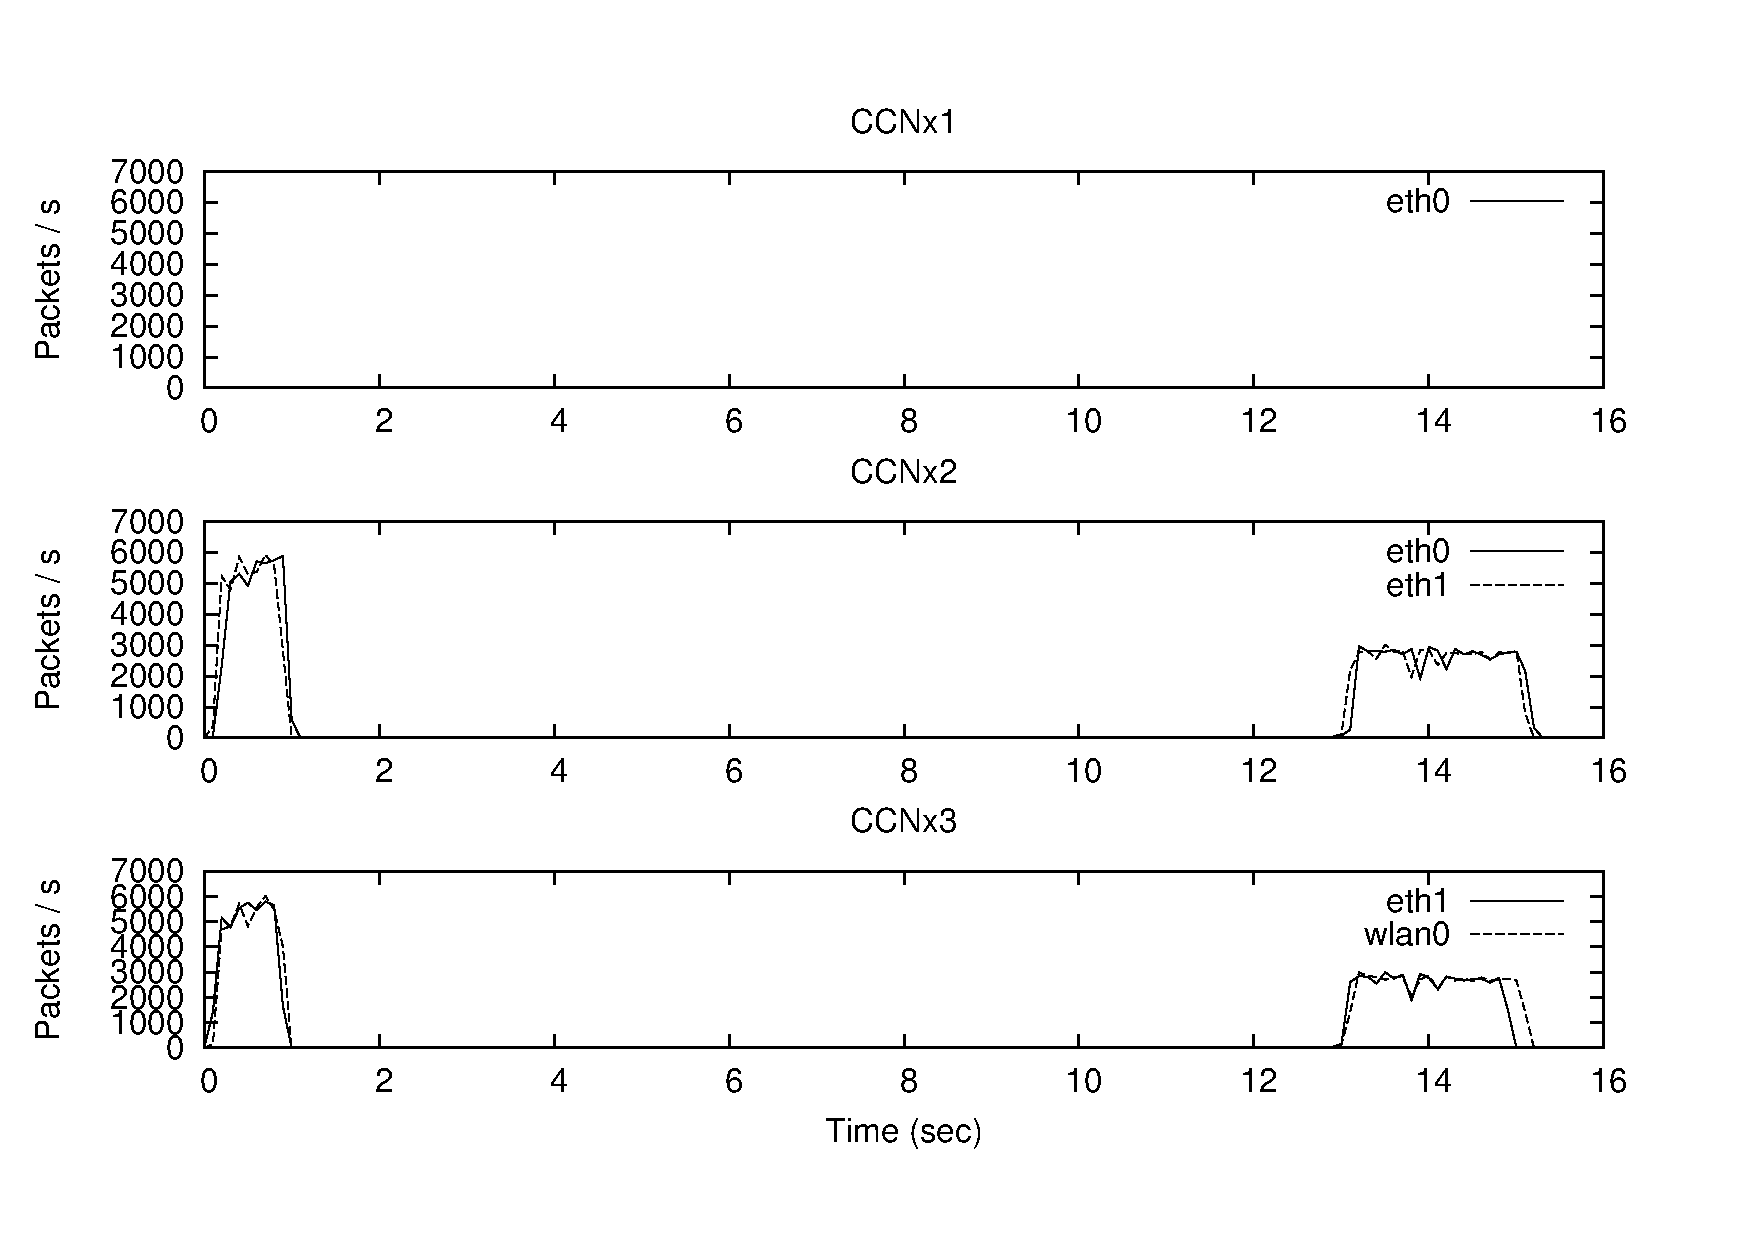
\includegraphics[width=0.75\textwidth] {figures/file_5-ctrl-net.pdf}
        \label{subfig:file_5-ctrl-net}
    }

    \subfigure[]{
        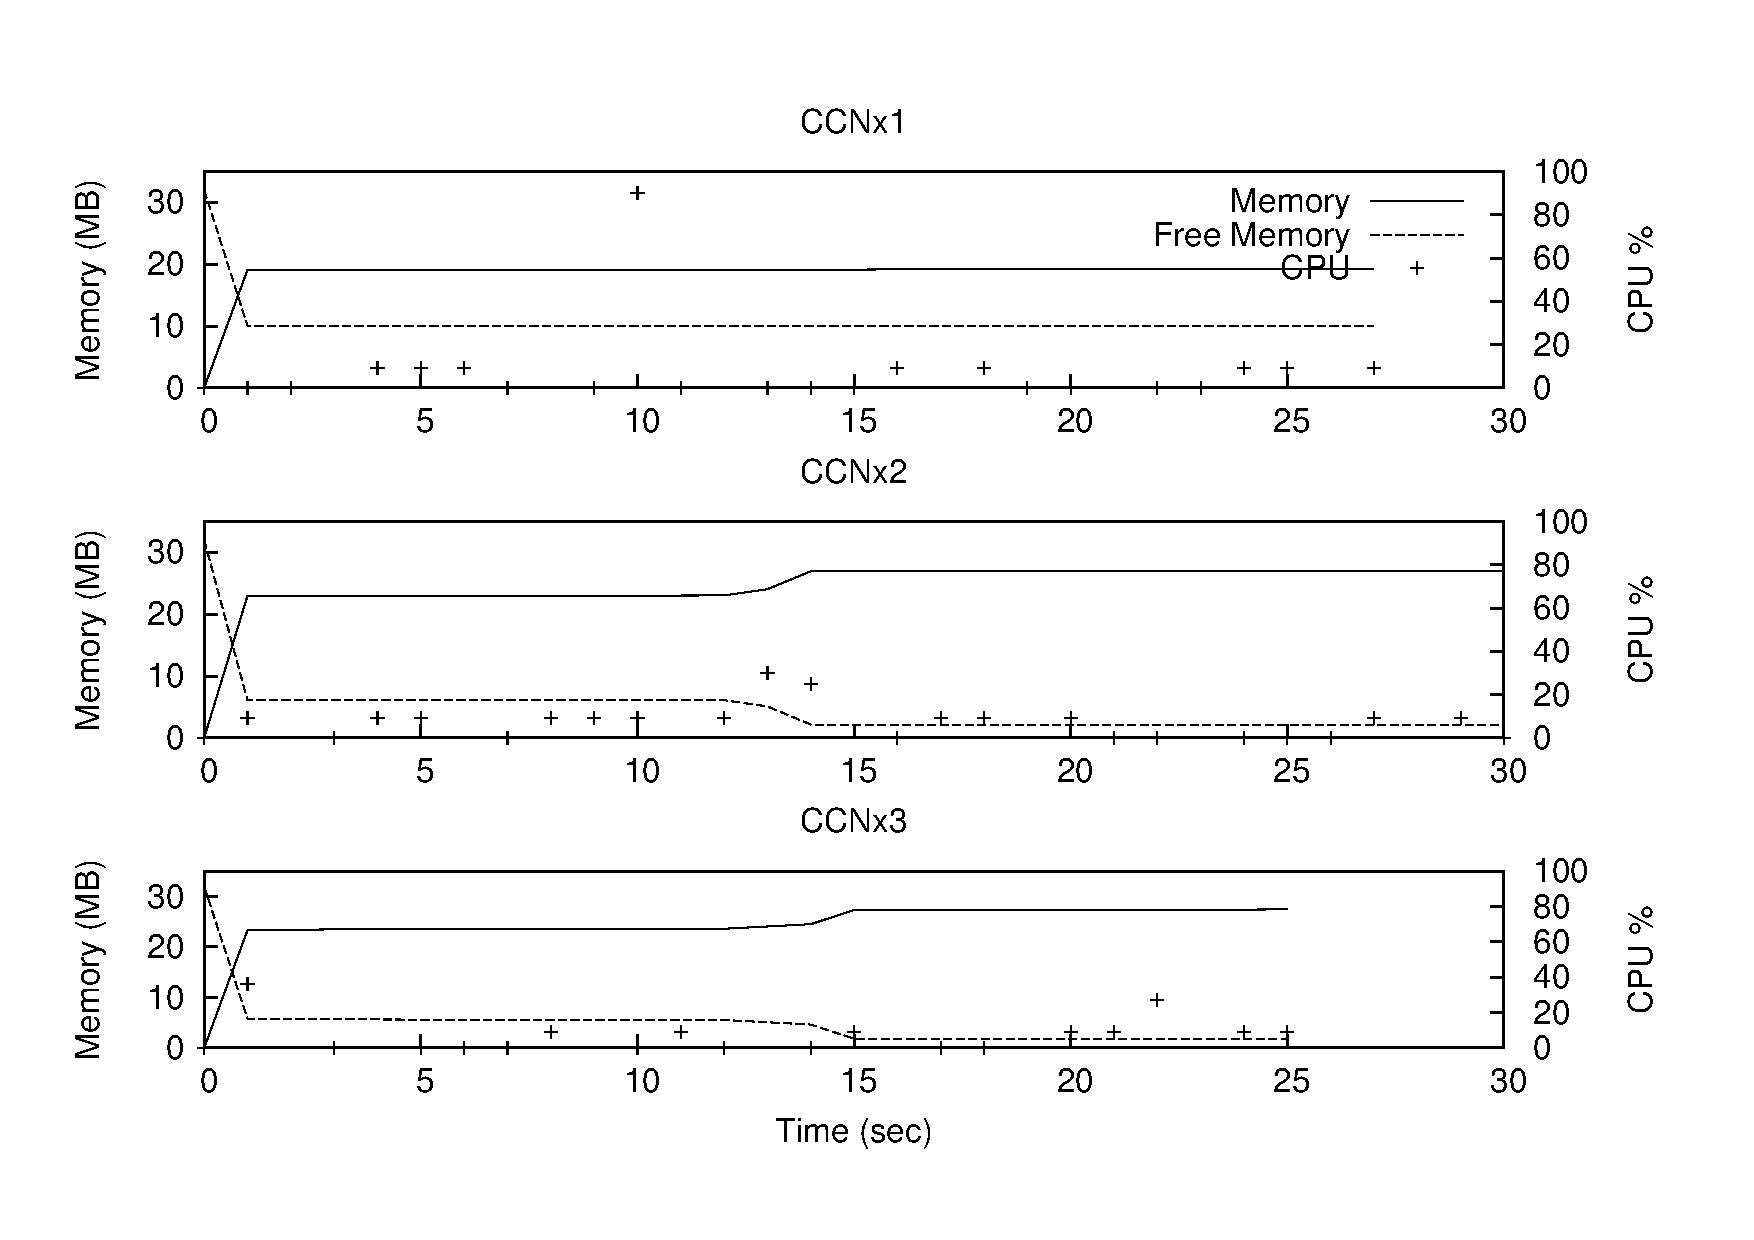
\includegraphics[width=0.75\textwidth] {figures/file_5-ctrl-cpu-mem.pdf}
        \label{subfig:file_5-ctrl-cpu-mem}
    }

    \cprotect\caption{Results for Test 2.1: Network load (a) and 
        CPU and memory utilization (b) at 
        all routing nodes, during the transfer of a file of size 
        5\,MB over FTP, for a non-overlapping case. Regarding the 
        memory values, the `memory' line corresponds to the amount of RAM 
        occupied by the \verb+ccnd+ process, while the `free memory' corresponds 
        to the amount of free memory in the system.}
    \label{fig:file_5-ctrl}

\end{figure}

\subsection{Test 2.2 - CCNx Multihop Forwarding (Video Streaming)}
\label{subapp:test-multihop-video}

\begin{figure}[H]
    \centering

    \subfigure[]{
        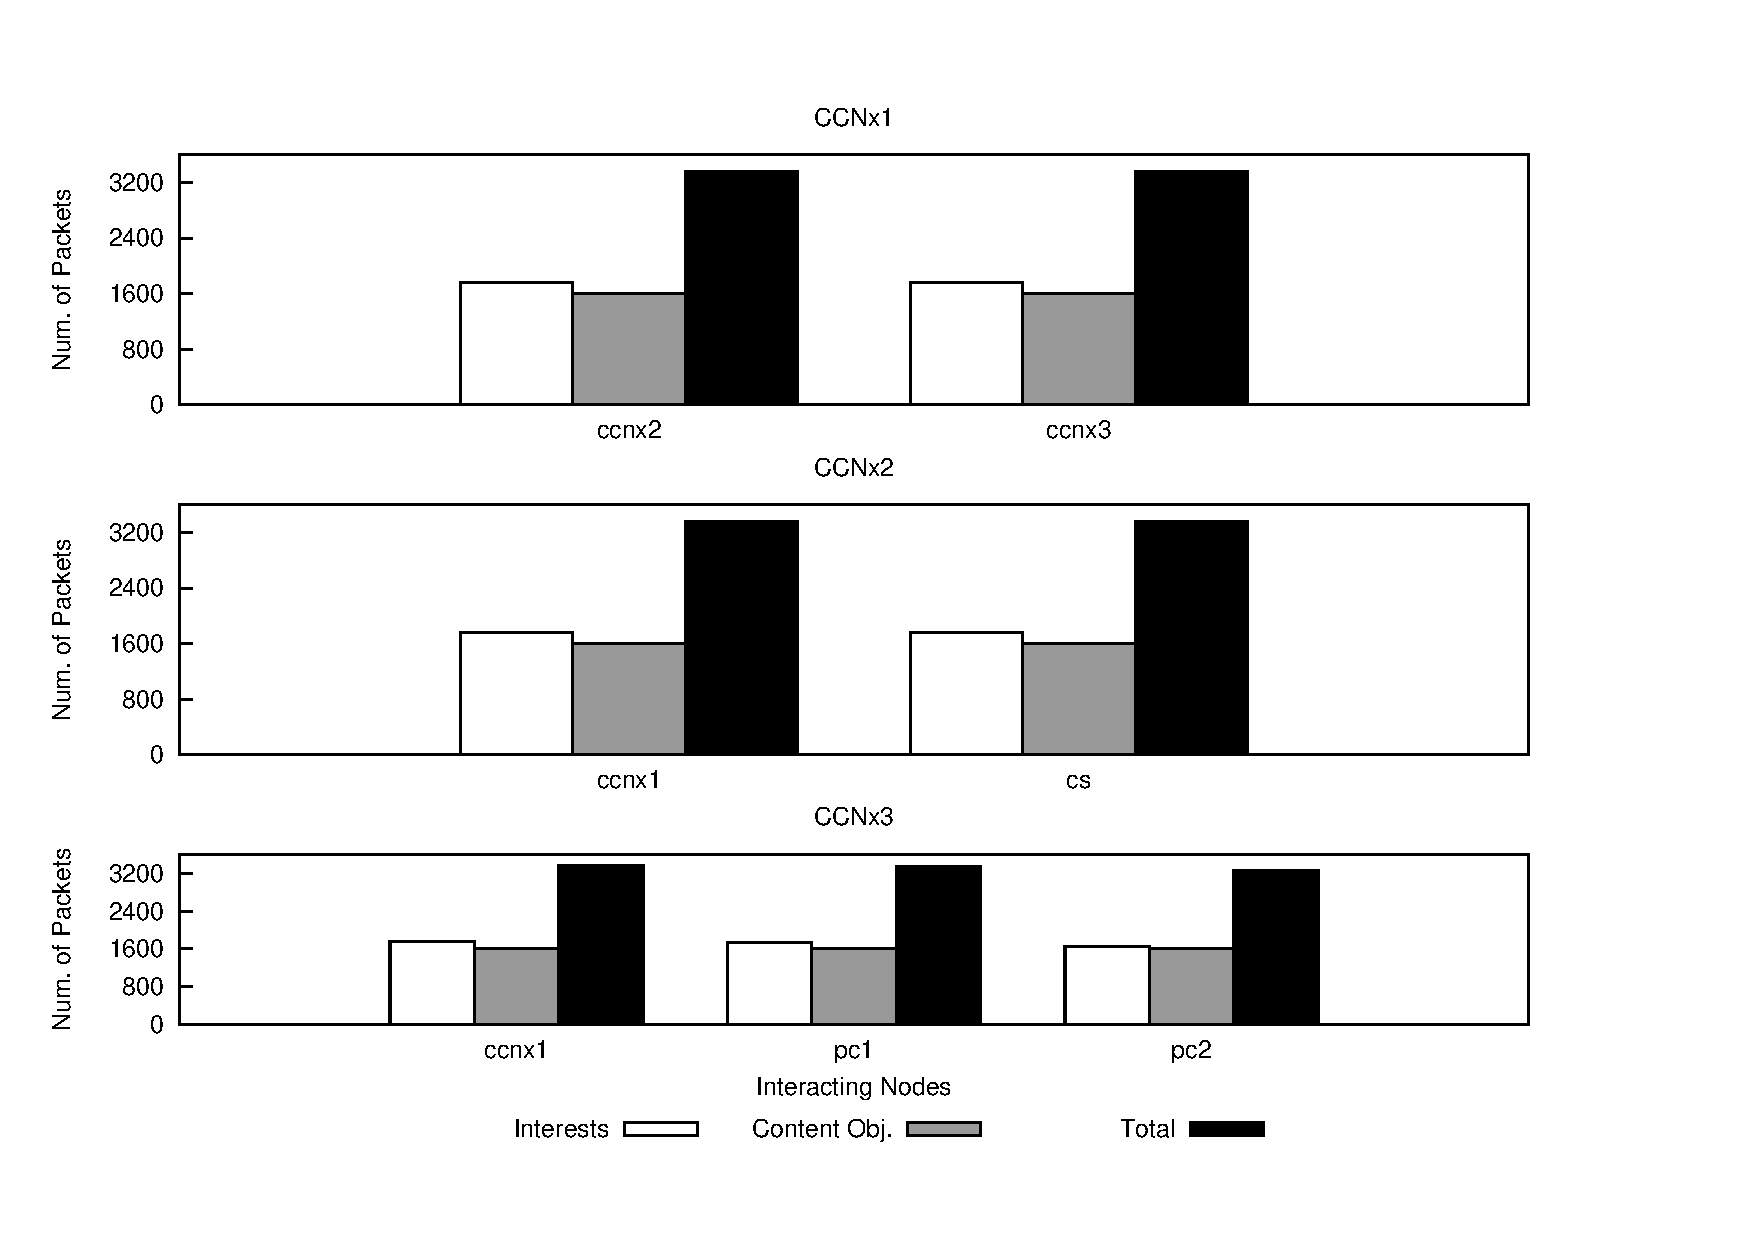
\includegraphics[width=0.75\textwidth] {figures/video-sep-pckt.pdf}
        \label{subfig:video-sep-pckt}
    }

    \subfigure[]{
        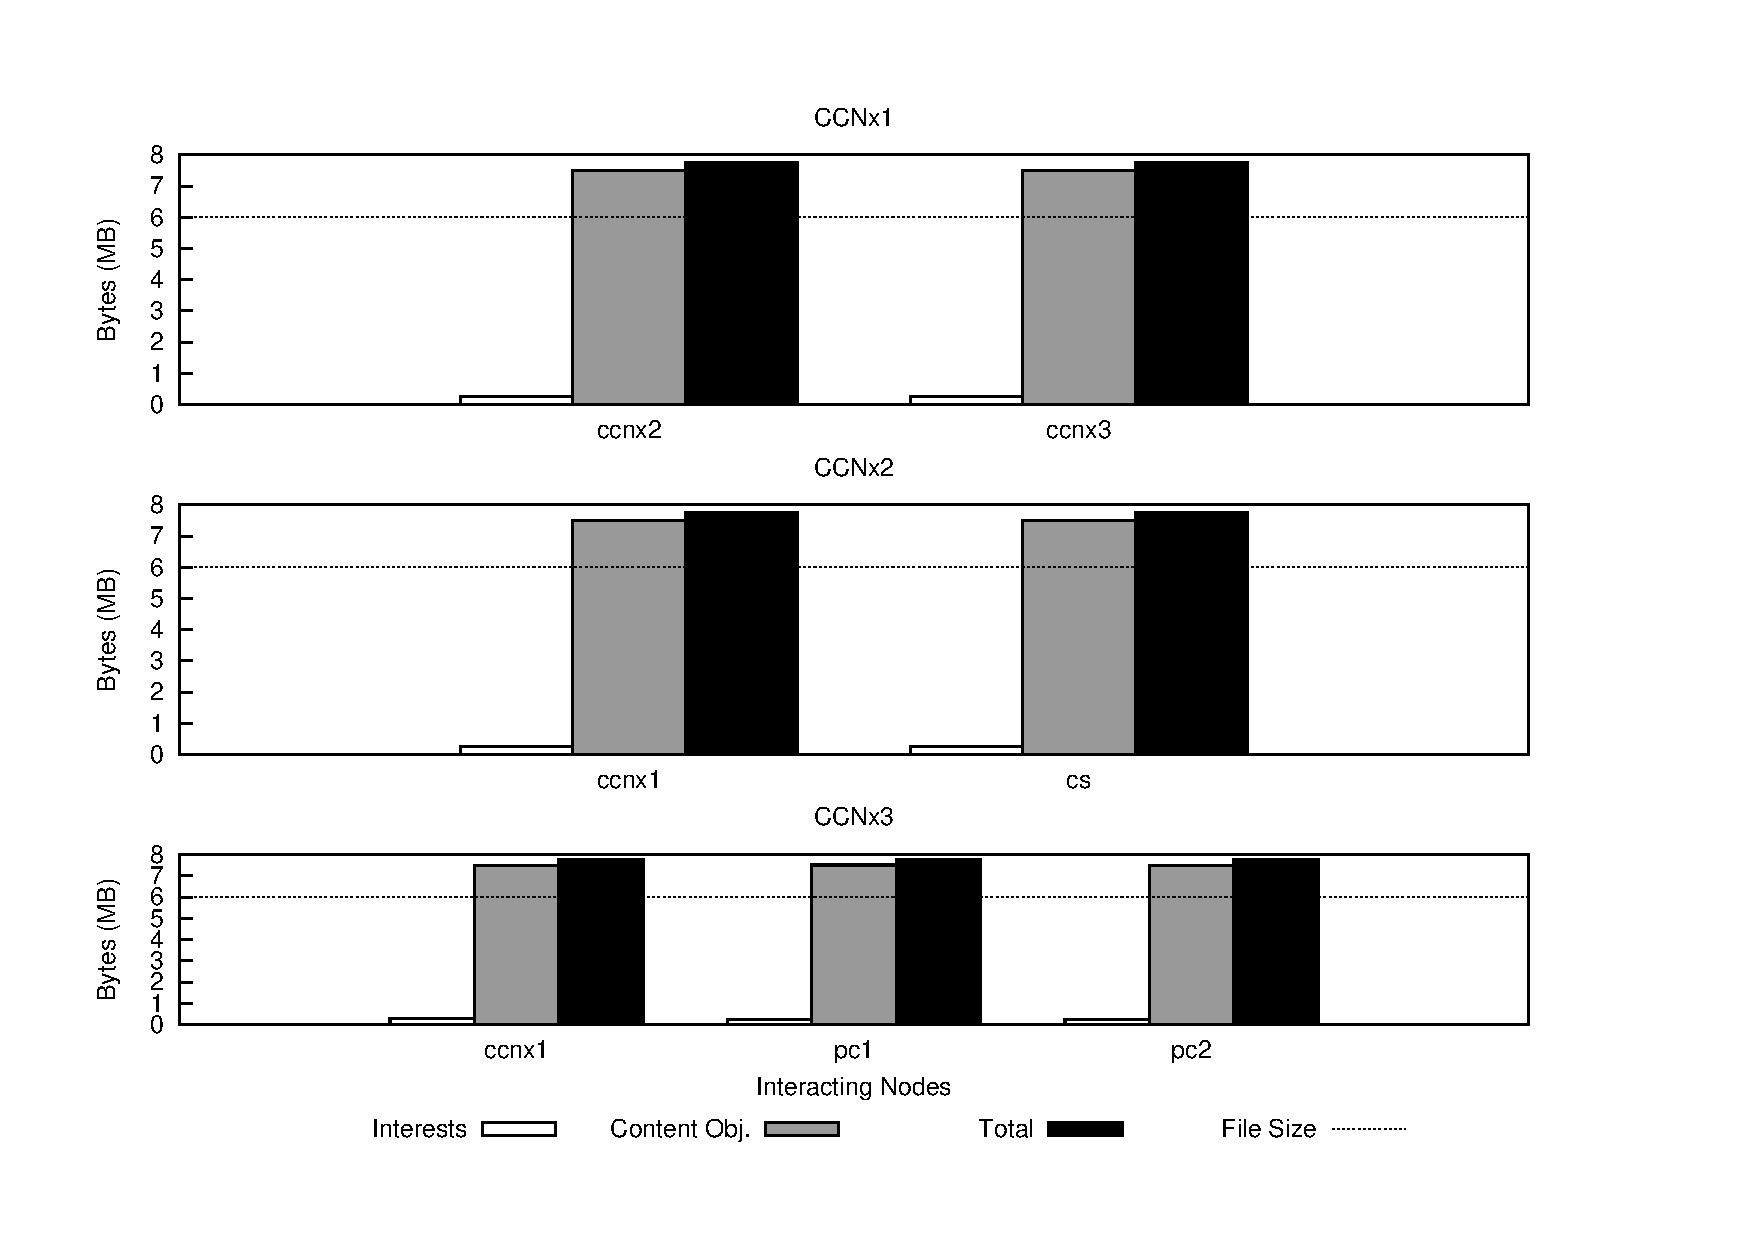
\includegraphics[width=0.75\textwidth] {figures/video-sep-byte.pdf}
        \label{subfig:video-sep-byte}
    }

    \cprotect\caption{Results for Test 2.2: Packet (a) and byte (b) 
        counts (Interest and 
        Content Objects) registered at each CCNx forwarding node, exchanged 
        between the respective peer elements. This test involves the 
        streaming of a video of size 6.3\,MB and 8 seconds duration from 
        the content source CS to nodes PC1 and PC2 (see Figure~\ref{fig:basic-testbed}).}
    \label{fig:video-sep-abs}

\end{figure}

\begin{figure}[H]
    \centering

    \subfigure[]{
        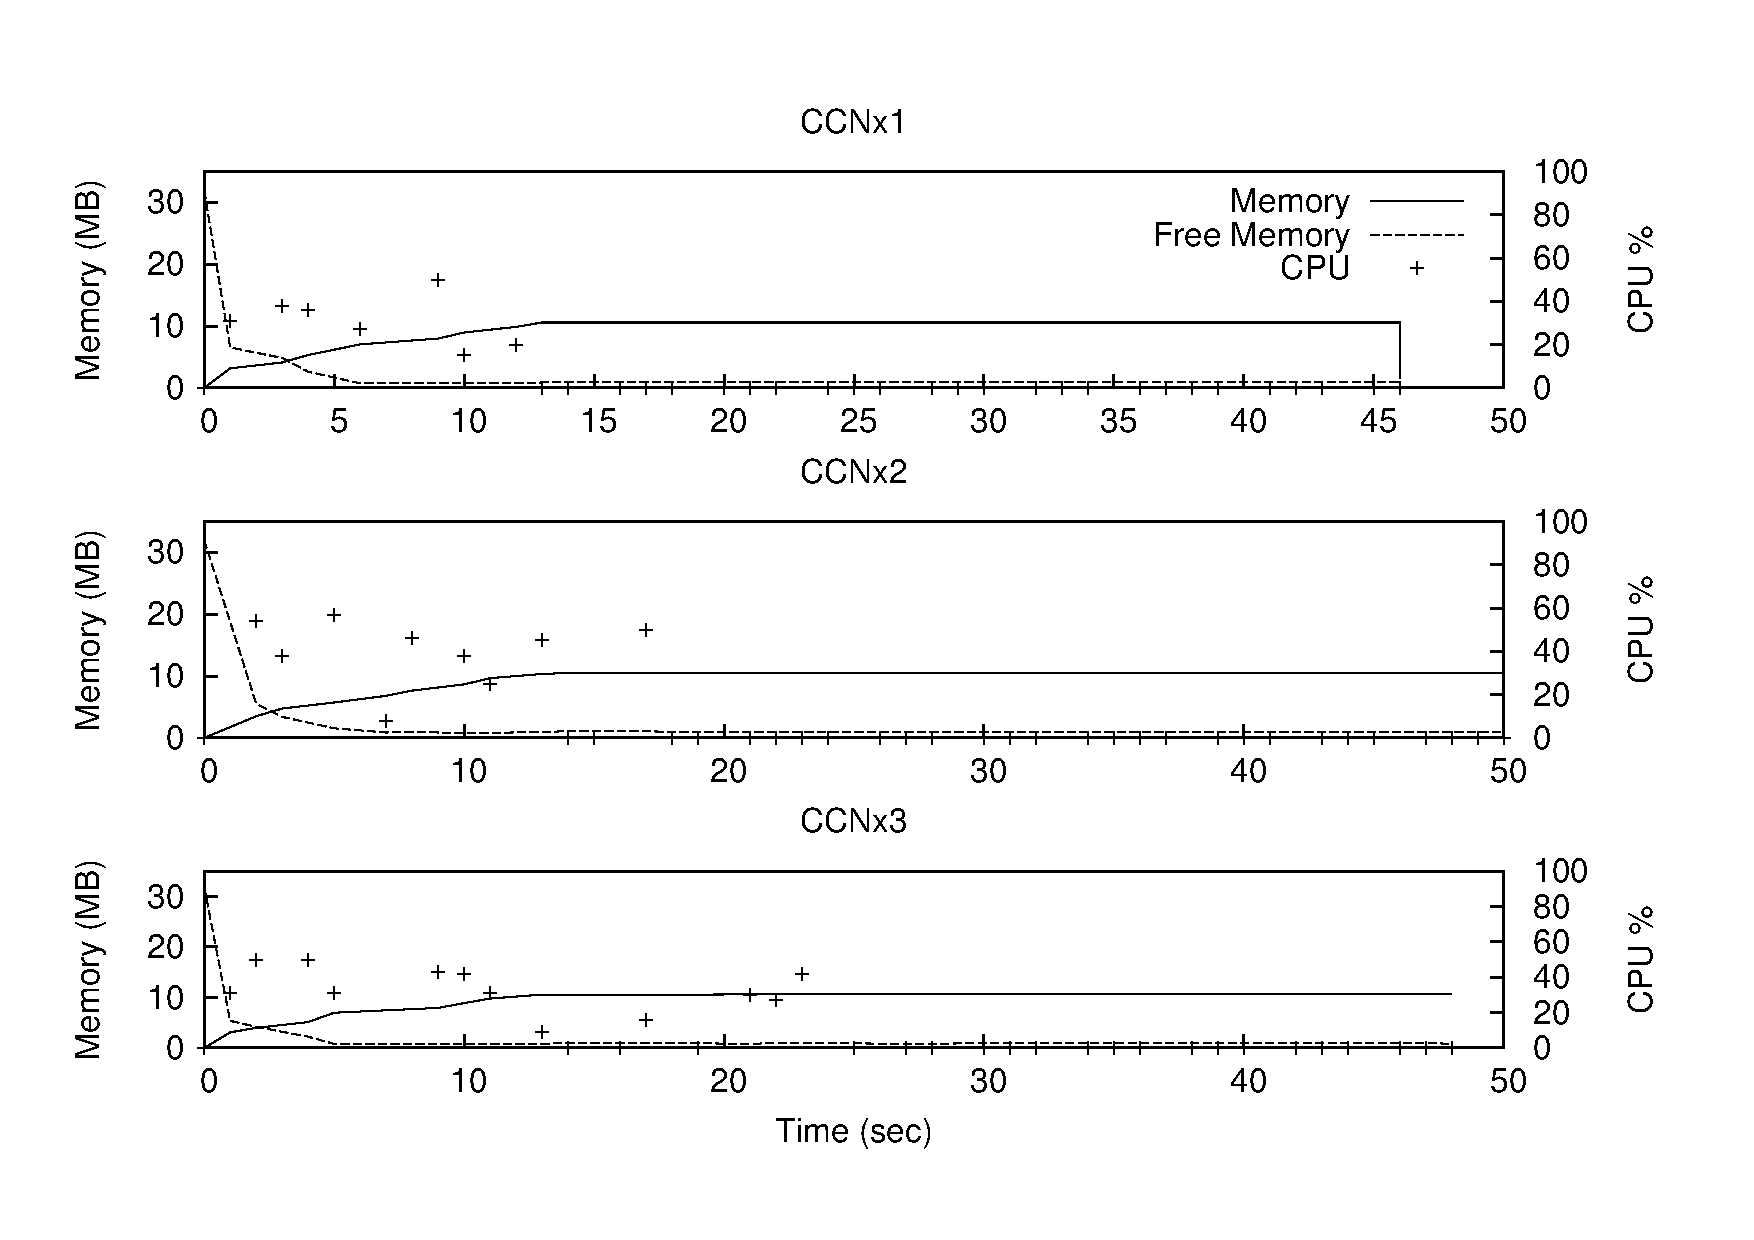
\includegraphics[width=0.75\textwidth] {figures/video-sep-cpu-mem.pdf}
        \label{subfig:video-sep-cpu-mem}
    }

    \subfigure[]{
        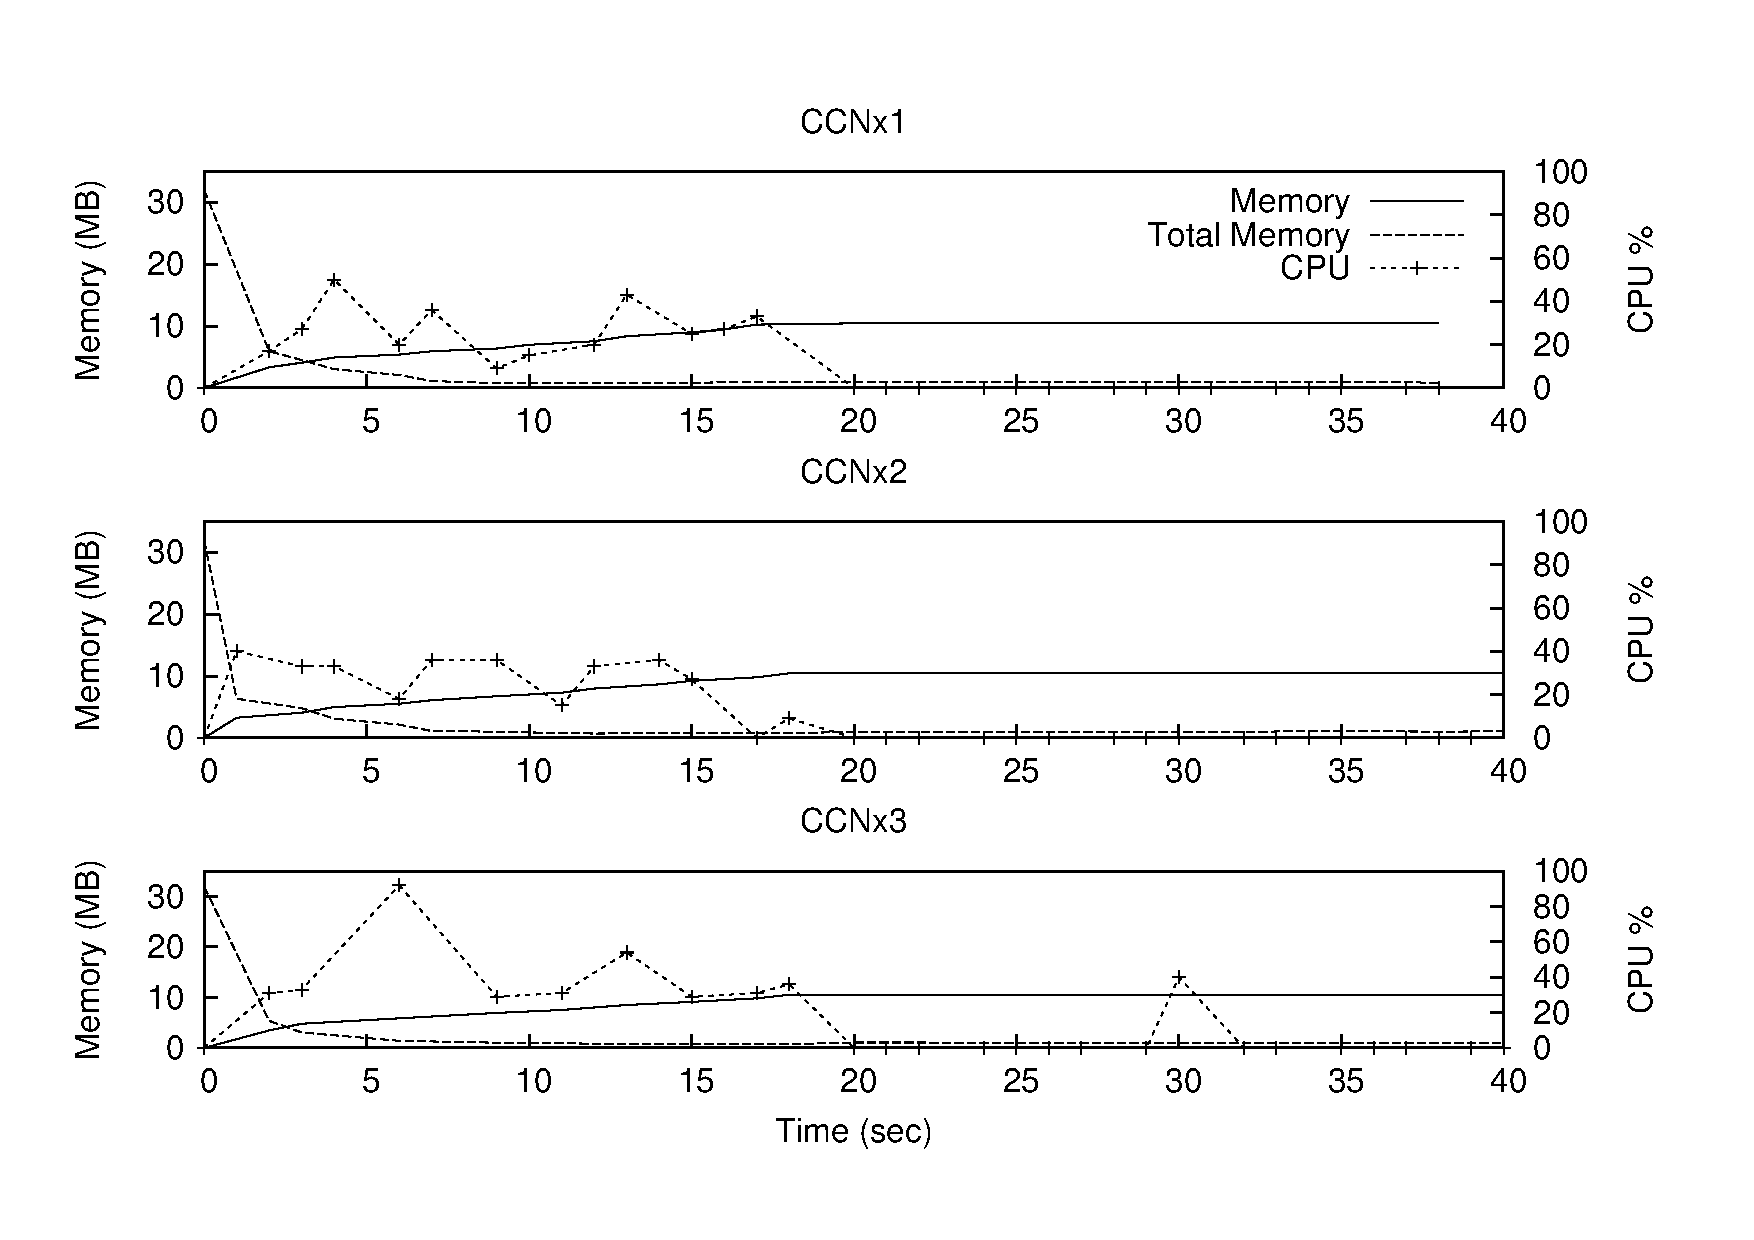
\includegraphics[width=0.75\textwidth] {figures/video-sim-cpu-mem.pdf}
        \label{subfig:video-sim-cpu-mem}
    }

    \cprotect\caption{Results for Test 2.2: CPU and memory utilization at 
        all CCNx nodes, during the streaming of a video file of size 
        6.3\,MB and 8 second duration, for both non-overlapping (a) and 
        overlapping (b) cases. Regarding the 
        memory values, the `memory' line corresponds to the amount of RAM 
        occupied by the \verb+ccnd+ process, while the `free memory' corresponds 
        to the amount of free memory in the system.}
    \label{fig:video-cpu}

\end{figure}

\subsection{Test 2.3 - CCNx Multihop Forwarding (Multiple Paths)}
\label{subapp:test-multihop-multipath}

\begin{figure}[H]
    \centering

    \subfigure[]{
        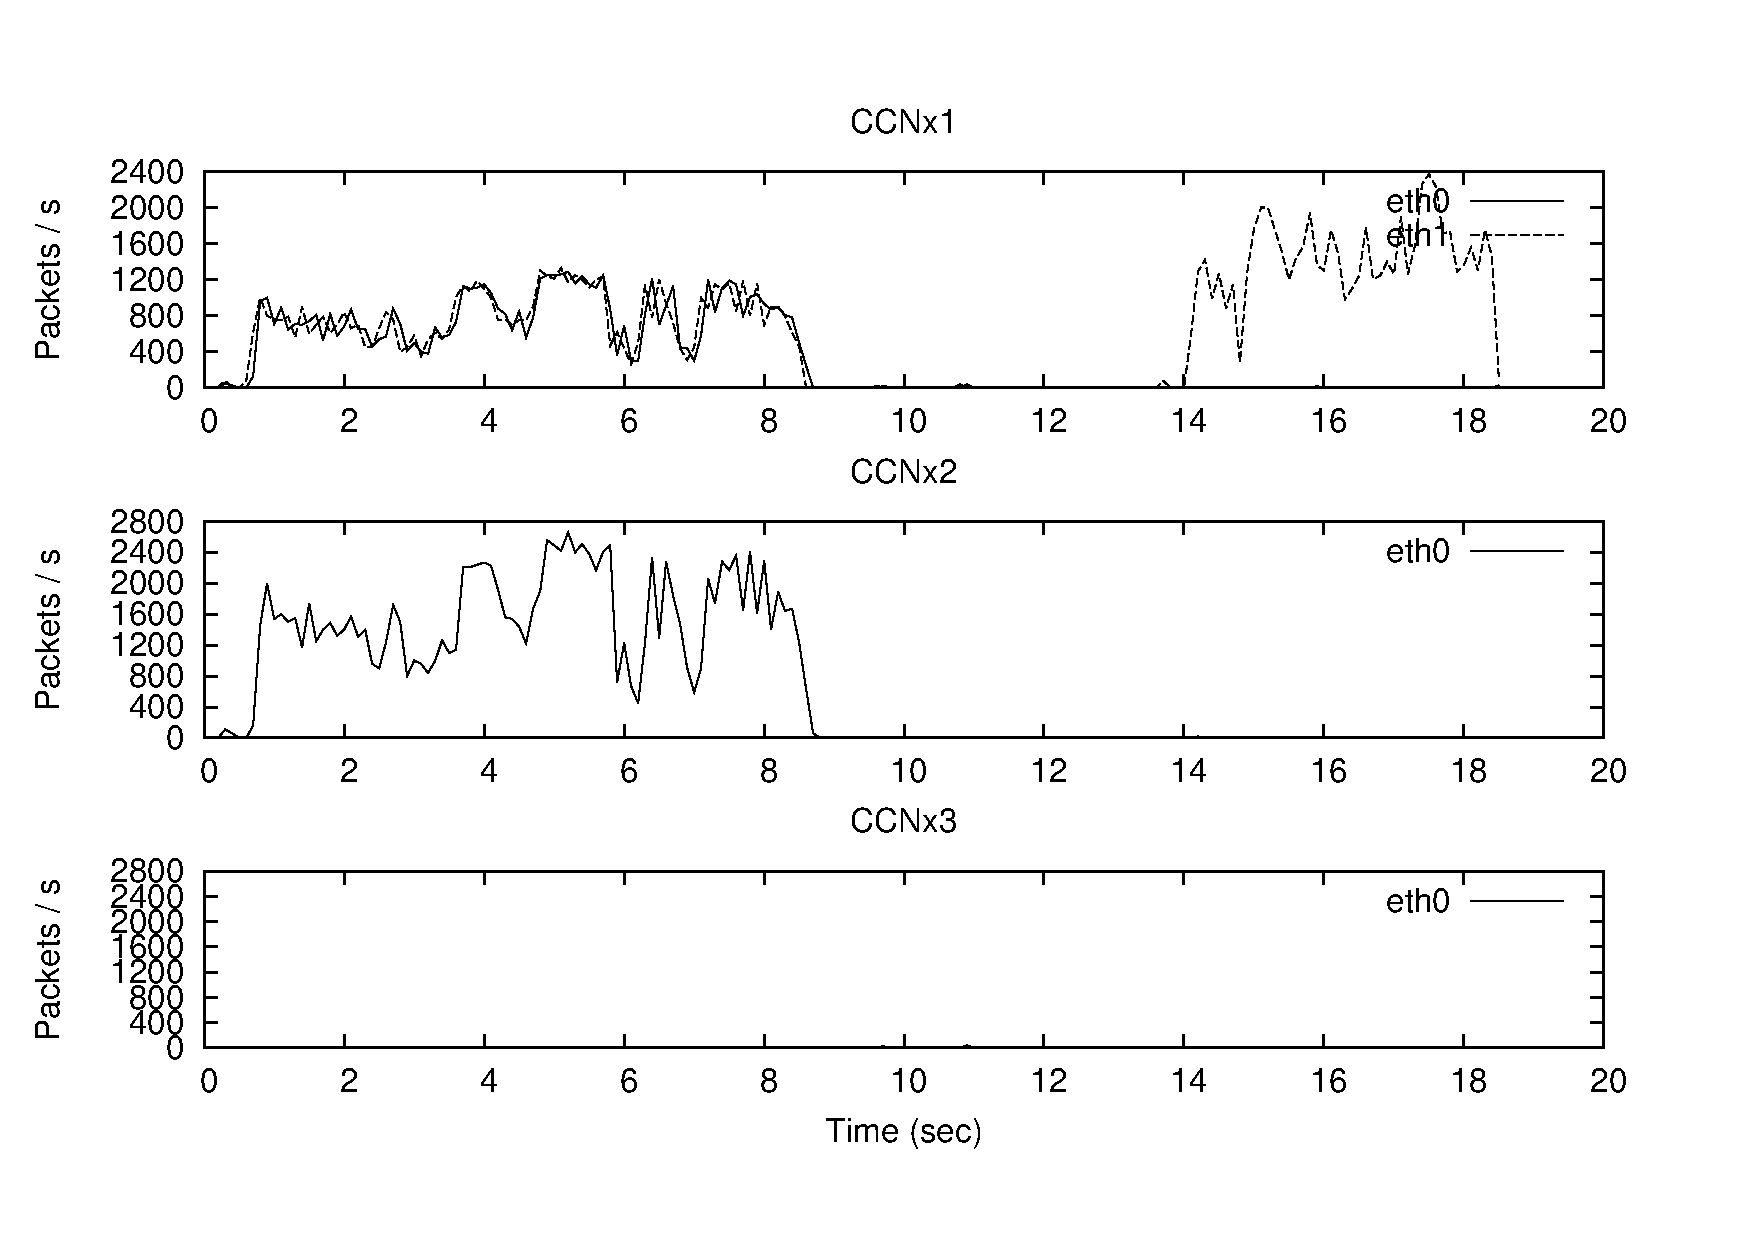
\includegraphics[width=0.75\textwidth] {figures/short-route-net.pdf}
        \label{subfig:short-route-net-app}
    }

    \cprotect\caption{Results for Test 2.3: Network load at 
        all CCNx nodes, during the transfer of a file of size 5\,MB 
        (non-overlapping case), using the `short' path indicated in 
        Figure~\ref{fig:testbed-multiple-paths}.}
    \label{fig:short-route-app}

\end{figure}

\begin{figure}[H]
    \centering

    \subfigure[]{
        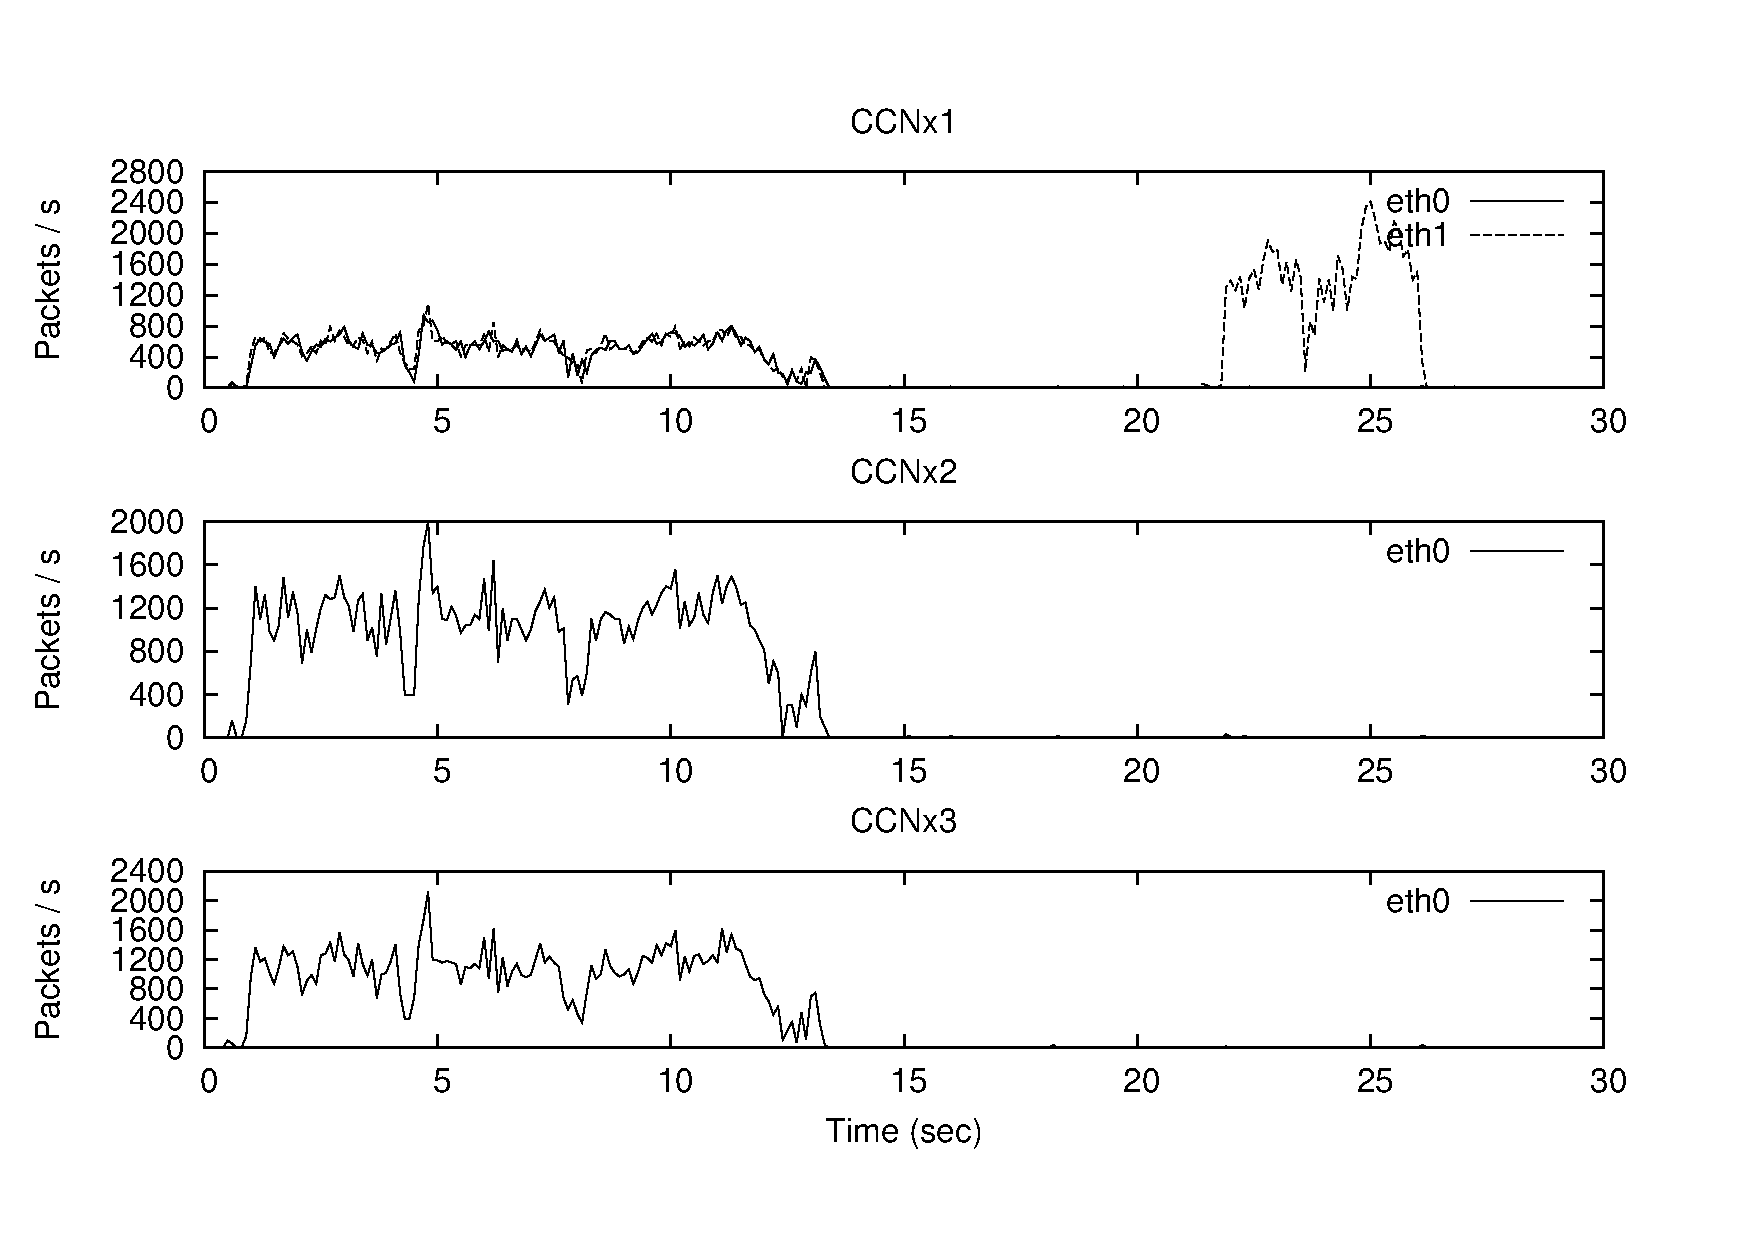
\includegraphics[width=0.75\textwidth] {figures/long-route-net.pdf}
        \label{subfig:long-route-net-app}
    }

    \subfigure[]{
        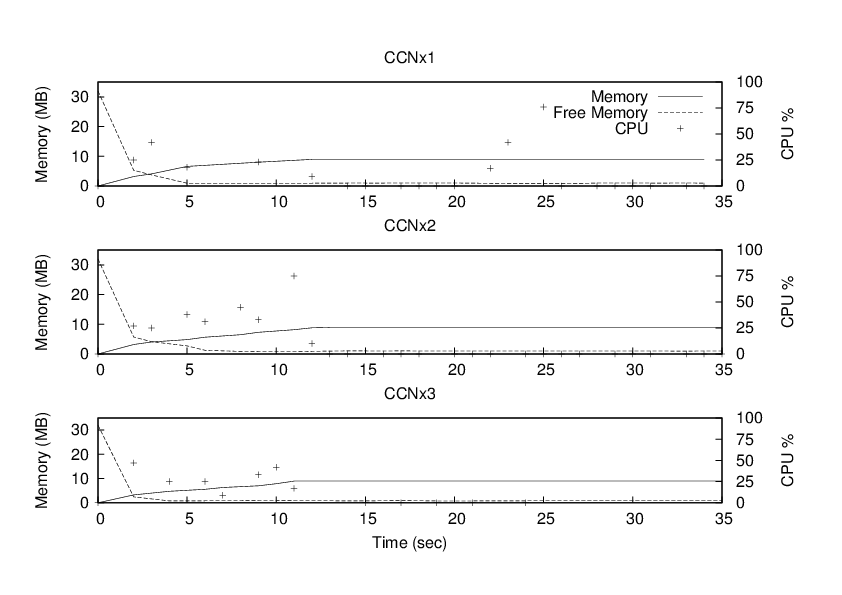
\includegraphics[width=0.75\textwidth] {figures/file_5-long-route-cpu-mem.pdf}
        \label{subfig:long-route-app}
    }

    \cprotect\caption{Results for Test 2.3: Network load (a) and and 
        CPU and memory utilization (b) at 
        all CCNx nodes, during the transfer of a file of size 5\,MB 
        (non-overlapping case), using the `long' path indicated in 
        Figure~\ref{fig:testbed-multiple-paths}. Regarding the 
        memory values, the `memory' line corresponds to the amount of RAM 
        occupied by the \verb+ccnd+ process, while the `free memory' corresponds 
        to the amount of free memory in the system.}
    \label{fig:long-route-app}

\end{figure}

\begin{figure}[H]
    \centering

    \subfigure[]{
        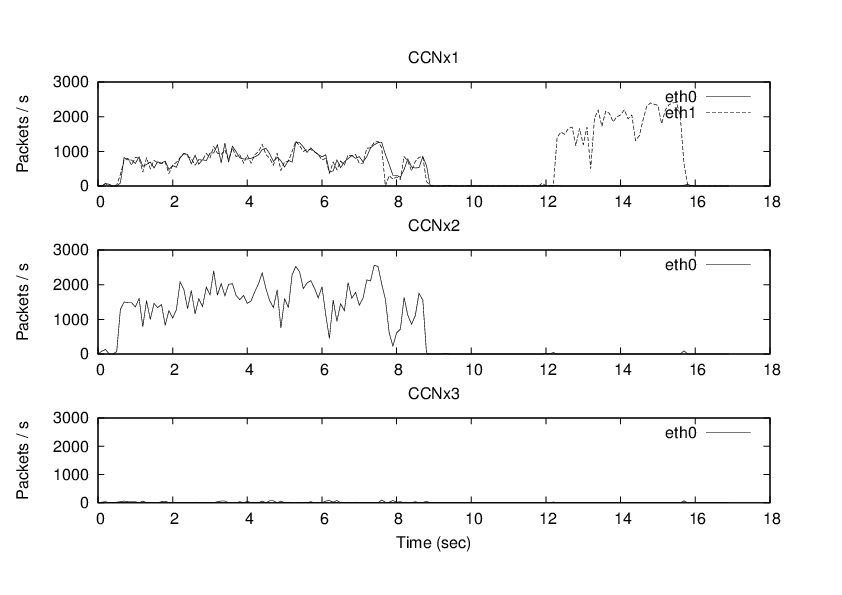
\includegraphics[width=0.75\textwidth] {figures/long-short-route-net.pdf}
        \label{subfig:long-short-route-net-app}
    }

    \subfigure[]{
        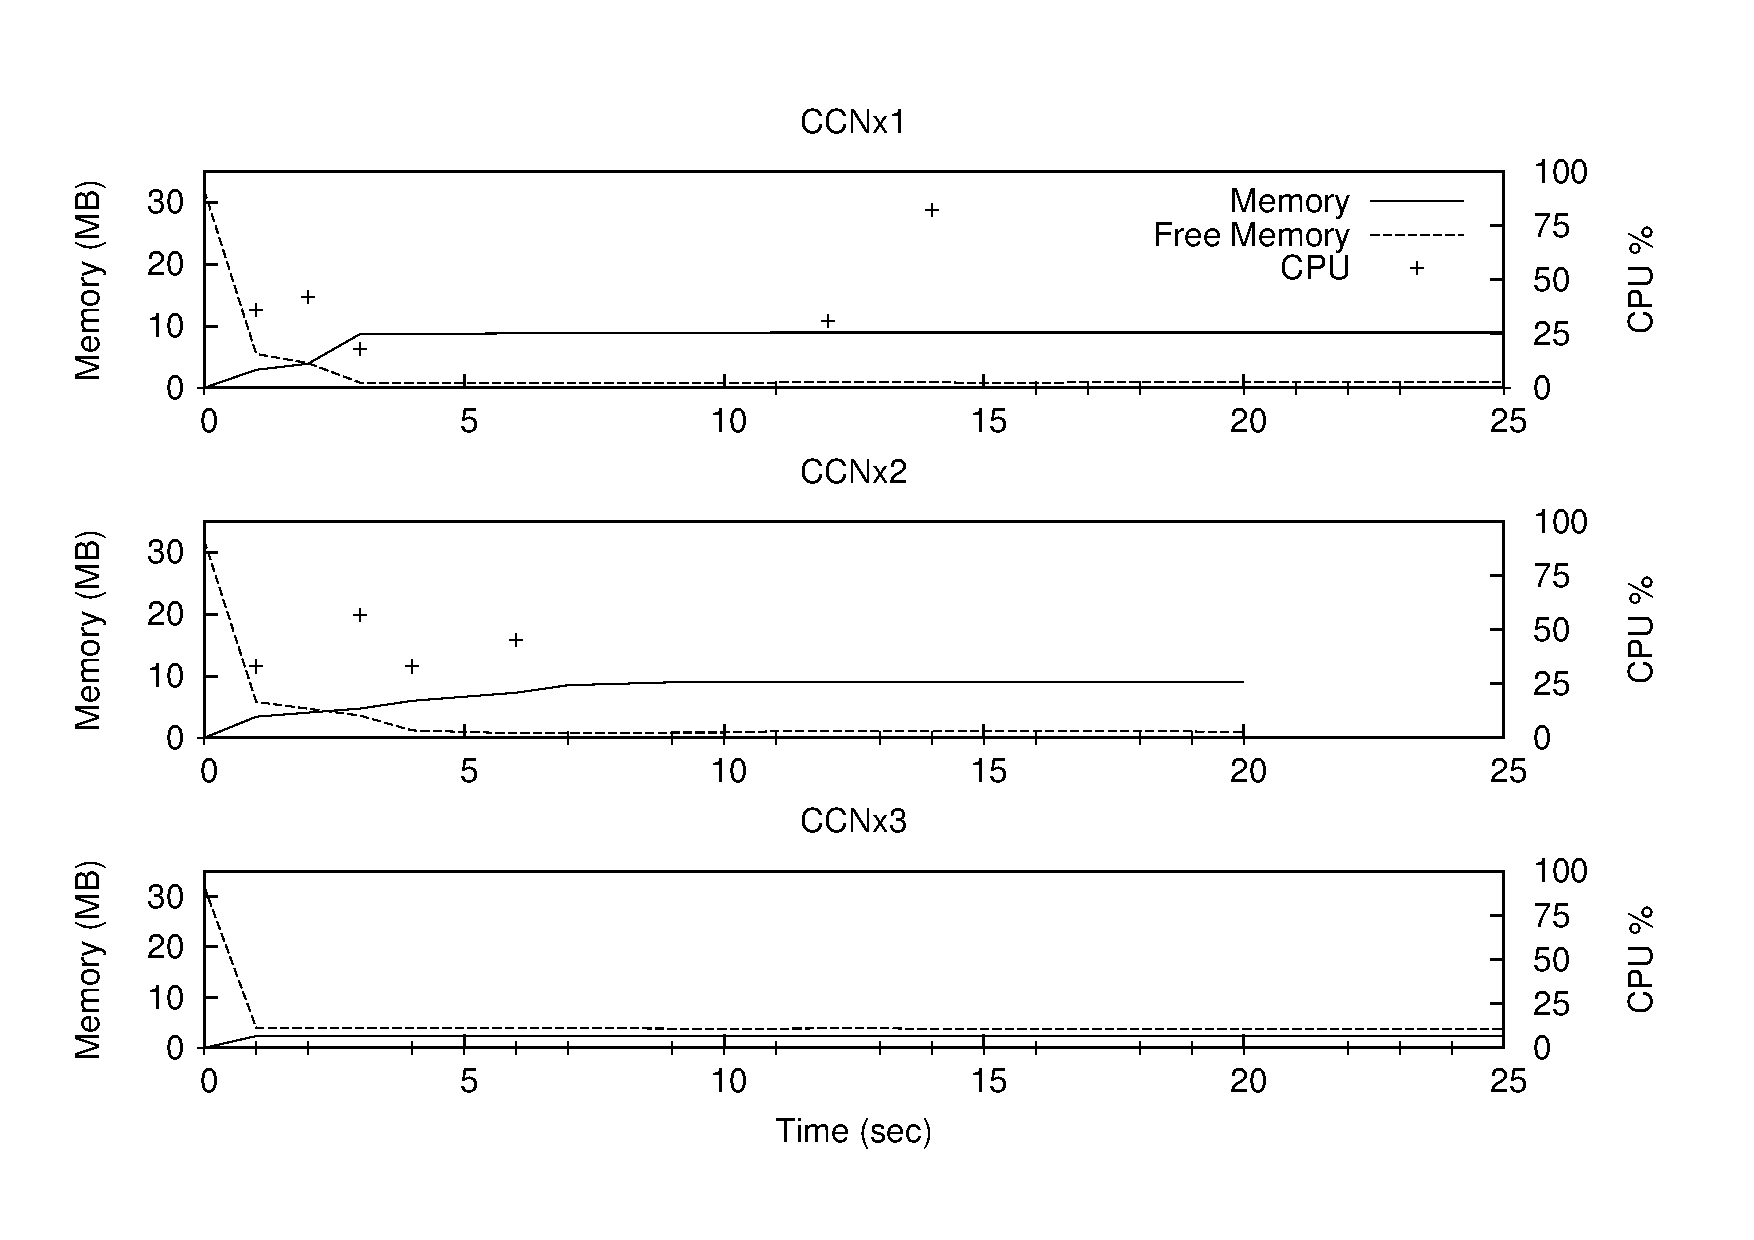
\includegraphics[width=0.75\textwidth] {figures/file_5-long-short-route-cpu-mem.pdf}
        \label{subfig:long-short-route-app}
    }

    \cprotect\caption{Results for Test 2.3: Network load (a) and and 
        CPU and memory utilization (b) at 
        all CCNx nodes, during the transfer of a file of size 5\,MB 
        (non-overlapping case), using both `short' and `long' paths indicated in 
        Figure~\ref{fig:testbed-multiple-paths}. Regarding the 
        memory values, the `memory' line corresponds to the amount of RAM 
        occupied by the \verb+ccnd+ process, while the `free memory' corresponds 
        to the amount of free memory in the system.}
    \label{fig:long-short-route-app}

\end{figure}

